\chapter{Landscape-wide land changes correlate with, but rarely explain local bird diversity change}
%\addcontentsline{toc}{chapter}{Chapter 3}
%\markboth{}{Impacts of past abrupt land change on local biodiversity globally}
\label{C05}

There is an ongoing debate whether biodiversity at local scales is changing and what might drive these changes. Land changes are suspected to impact local biodiversity change. However, there is little evidence across spatial and temporal scales and for multiple functional groups of species, thus limiting our understanding of the drivers of local biodiversity change. Here we investigate whether landscape-wide land changes, opposed to those at the local scale, are driving local bird diversity change. We link time series of 34 years of breeding bird survey (BBS) data (1984-2017) at 2745 routes across the continental United States of America with remotely-sensed satellite imagery (\textasciitilde30m resolution) from the Landsat missions. Specifically, we assessed for each year what proportion of the landscape surrounding the BBS routes had a land change \textendash\ defined as abrupt shift in magnitude or trend of photosynthetic activity as detected by the Breaks for Additive Seasonal and Trend (BFAST) algorithm \textendash\ and tested whether large proportions of concurrent or preceding landscape-wide land changes explain changes in bird diversity, quantified as either geometric mean of relative abundance (GM) or progressive Bray-Curtis index (pBC). We found that the GM was negatively and the pBC positively correlated with a large proportion of land changes in the wider landscape. Furthermore, the consideration of preceding \textendash\ instead of concurrent \textendash\ landscape-wide land changes explained on average more variation in bird diversity change. Overall, landscape-wide land changes failed to explain most of the variation in local bird diversity change for most BBS routes regardless if bird diversity change is differentiated by functional groups or geographic regions. This study is one of the first studies attempting to link land and biodiversity change. It highlights the influence of preceding and concurrent land change on biodiversity and makes suggestions for promising directions of future research.  

\section{Introduction}
\label{C05_01}

Ongoing human alteration of the Earth surface causes changes in biodiversity across scales \citep{Gibson2011,Murphy2014,Newbold2015}. Globally, about 32\% of all known vertebrate species show decreasing population sizes and range contractions \citep{Ceballos2017,WWF2018} with reported species extinction rates being several times higher than expected naturally \citep{Brooks2002,Pimm2014}. Yet, any change in biodiversity is scale and measure dependent \citep{Sax2003,Chase2013} and, perhaps surprisingly, there is still a debate whether local \textendash\ opposed to global \textendash\ biodiversity is truly changing \citep{Thomas2013,McGill2014}. 

A number of global meta-analyses demonstrated that some biodiversity measures, notably species richness, have not changed at the local scale \citep{Vellend2013,Vellend2017,Dornelas2014}. However, these results have been questioned, particularly on whether the data are spatially and temporally biased \citep{Gonzalez2016} or if sites with and without land change were differentiated \citep{Cardinale2018}. This raises the question whether changes on land can explain changes in local biodiversity measures across space and time. 

Present differences on land influence local biodiversity globally. Previous studies found local biodiversity to be consistently reduced at sites with more intensively used land \citep{Murphy2014,Newbold2015,Alroy2017}, where on average 13.6\% fewer species and 10.7\% fewer individuals were observed compared to undisturbed "primary vegetation" \citep{Newbold2015}. However, these analyses relied on spatial comparisons of local biodiversity and therefore do not capture temporal biodiversity change \textit{per se}. In addition, they ignored the influence of past land changes \citep{Perring2018,Jung2018} and did not consider landscape-wide land changes, which can influence local biodiversity \citep{Tscharntke2012,Turner2015,Miguet2015}. 

Local biodiversity is influenced by the variability of resources, such as food or nesting material, or through ecological processes, such as migration or fear of predation, at the landscape scale \citep{Hanski2000,Chase2003,Turner2015,Fernandez2016}. However these influences are not static and landscapes are constantly changing because of natural and anthropogenic factors \citep{Pickett1985,Manning2009,Turner2015}. Previous studies have shown that landscape-wide land changes may have a lasting influence on local biodiversity through ‘biotic lag’ effects \citep{Metzger2009,Ewers2013}. Yet, most studies focussed on small geographic regions and changes in forest cover \citep{Rittenhouse2010} and did not investigate general impacts of landscape-wide land changes on local biodiversity across spatio-temporal scales. A lack of data on local biodiversity and landscape-wide land change has so far prevented comparative assessments \citep{DePalma2018}.

Increasing availability of satellite imagery enables to quantify land change at broad spatial and temporal scales \citep{Kennedy2014,Pasquarella2016}. Long-running satellite missions, such as Landsat, provide one of the best sources to monitor land-surface conditions \citep{Kennedy2014,Vogelmann2016,Hermosilla2018,Song2018}. Time series of land-surface conditions, such as photosynthetic activity, can measure intra- and inter-annual vegetation dynamics \citep{Pettorelli2005,Fisher2006} and specific algorithms have been developed to detect land changes as changes in photosynthetic activity \citep{Verbesselt2010,Zhu2017}. Land changes can be differentiated by attributes \citep{Watson2014}, such as abrupt shifts in magnitude, causing an immediate loss or gain of vegetation \citep{DeVries2015b}, or shifts in trend, causing either greening or browning over time \citep{dejong2013,Muller2014}. These attributes can be robustly quantified at the landscape scale and linked to changes in local biodiversity.

Birds are one of the best surveyed taxonomic groups globally. Local biodiversity change quantified from repeated breeding bird surveys (BBS) has been widely studied \citep{Harrison2014,Pardieck2018}. Previous studies have shown that changes in bird diversity are dependent on the specific biodiversity measure     considered \citep{Schipper2016,Jarzyna2017} and are often non-linear \citep{Gutzwiller2015,Barnagaud2017}. Bird diversity change also varied spatially \citep{Harrison2014,Jarzyna2017} with many birds of particular functional traits, such as migratory or grassland dependent species, declining in developed countries \citep{Fewster2000,Sanderson2006,Stanton2018}. Land changes are most likely a driving factor of these declines \citep{Harrison2014,Harrison2016}, and yet most previous studies using BBS data investigated only spatial correlations between remotely-sensed attributes of land change and local bird diversity \citep{Rowhani2008,Goetz2014,Hobi2017}. Notably \cite{Rittenhouse2010} found bird assemblage composition to be altered in landscapes with more “disturbed forests”, which they assessed using remotely-sensed time series. However, to our knowledge, no previous study has investigated whether landscape-wide land changes correlate with and explain changes in local bird diversity.

Consequently, this study hypothesizes that (\textit{i}) changes in local bird diversity are driven by landscape-wide land changes depending on their attributes, (\textit{ii}) local bird diversity change can best be explained by past land changes, and that (\textit{iii}) the explanatory power of landscape-wide land changes on local bird diversity change varies across geographic regions and functional groups of bird species. We combine 34 years (1984–2017) of annual BBS records collected at sites across the continental United States of America with time series of medium-high resolution (nominal \textasciitilde30m) satellite imagery from the Landsat missions. Using Breaks for Additive Seasonal and Trend (BFAST), a generic change detection algorithm, we detect abrupt shifts in magnitude (immediate gain or loss in photosynthetic activity) and trend (greening or browning) of photosynthetic activity in the landscape surrounding each BBS route. Non-linear spatio-temporal models were used to correlate the proportion of changing land in the wider landscape with changes in local bird diversity.

\section{Methods}
\label{C05_02}
\subsection{Bird diversity time-series preparation}
\label{C05_0201}

Time series of local bird count records (1984 – 2017) were obtained from the North American Breeding Bird Survey \citep[BBS, available from \href{https://www.pwrc.usgs.gov/bbs/}{https://www.pwrc.usgs.gov/bbs/},][]{Pardieck2018} dataset. Bird counts were conducted annually during the breeding season (April to August with > 83.3\% sampled in June) along approximately $39.4$km long roadside survey routes and usually follow a standard protocol that involves fifty $3$min stops at evenly spaced intervals (approximately $0.8$km) \citep{Ralph1995}. At each $3$min stop, volunteer observers record the number and identity of every bird species seen or heard within approximately $400$m distance from the route. For our analyses we only included routes that followed the standard BBS protocol of fifty randomly selected stops (94.4\% of all routes) and had at least ten years of sampling between 1984 and 2017, as many BBS routes were not sampled every year (mean proportion of missing years = 19.7\%). The period from 1984 to 2017 was chosen to align to the availability of satellite data (but see \ref{C05_0202}). We removed routes from the analyses with non-acceptable weather conditions according to BBS standards \citep{Ralph1995} and excluded all nocturnal, crepuscular and aquatic species from the analysis as they are not well sampled by BBS methods \citep{Gutzwiller2015,Jarzyna2017}. All partially identified species (e.g. “sp.”), hybrids and species with unclear taxonomy (\eg  “A x B”) were removed from further analyses. In total, time-series from 2745 routes (out of 5248 in the entire BBS dataset) had suitable data for further analyses.

We calculated two different biodiversity measures commonly applied to BBS data. First, we calculated the geometric mean of relative abundance (GM), which quantifies relative changes in both abundance and evenness \citep{Buckland2011,Buckland2017,Harrison2014}. The GM for the year $y$ is defined as $GM_{y} = \exp(\frac{1}{S} \sum_{i=1}^{S} \log(\frac{ A_{iy}+1 }{A_{iy_0}+1 })$), where $S$ quantifies the total number of species with $i$ being an individual species, $A_{iy}$ the abundance of species $i$ in year $y$. The GM is unaffected by species detectability as it is based on within-species abundance trends, however it cannot be quantified for absent species and is unable to reflect changes in assemblage composition \citep{Buckland2011}. We added a constant ($1$) to all abundance values before calculating the annual GM to account for the species being absent in some years. The first four years of BBS data (1984 – 1987) were used to define the baseline years $y_{0}$ (calculated from the median number of individuals for each observed species) and to align the analyses with the baseline years used in the land change detection (but see Methods \ref{C05_0203}). Whenever no BBS was conducted in the years between 1984 and 1987 on a given route, we used the first year of available BBS data to define the baseline year $y_0$. Second, as measure of changes in assemblage composition, we calculated the progressive Bray-Curtis index \citep[pBC, ][]{Bray1957,Rittenhouse2010} as the difference in composition between a baseline and all following years of sampled bird assemblages \citep{Rittenhouse2010}. The pBC is defined as $ = 1 - \sum_{i=1}^{S} \frac{ |A_{iy} - A_{iy_0}| }{ (A_{iy} + A_{iy_{0}}) } $, where $A_{iy}$ is the abundance of species $i$ in year $y$ and $A_{iy_{0}}$ the estimated abundance in the baseline $y_0$ (defined as for the GM, calculated from the median number of individuals for each observed species).


\subsection{Time series of annual photosynthetic activity at the landscape scale}
\label{C05_0202}

Following previous studies, we define the “landscape” as the $19.7$km radius buffer around the centroid of each BBS route because it fully encompasses the majority of BBS routes and approximates the median natal dispersal distance of North American bird species \citep{Sutherland2000,Pidgeon2007,Albright2011}. Grid cells with permanent open water, ice or snow cover were excluded using a land mask derived from the 2011 National Land Cover Database (NLCD) land-cover map at \textasciitilde 30m resolution \citep{Homer2015}. In addition, BBS routes with less than 50\% land area ($N = 18$) within the surrounding landscape were excluded from further analyses, assuming that in those routes breeding birds are less influenced by landscape-wide changes in terrestrial photosynthetic activity.

To quantify land changes in the landscape surrounding each BBS route, we used imagery from the Landsat 4, 5, 7 and 8 satellites (1984 to 2017, \textasciitilde 30m nominal resolution) supplied by the United States Geological Service (USGS) available through Google Earth Engine \citep{Gorelick2017}. All Landsat images were radiometrically \citep{Chander2009} and atmospherically calibrated to surface reflectances \citep{Masek2006}. For each surface reflectance image, we masked out non-land grid cells, including clouds and cloud shadows as identified by the ‘cFMask’ algorithm \citep{Zhu2012}, areas permanently covered with water \citep[> 90\% water occurrence probability in the period 1984 – 2016, ][]{Pekel2016}. A spectral index of photosynthetic activity \citep[the two-band enhanced vegetation index (EVI),][]{Jiang2008} was calculated for each surface reflectance image. We composited all EVI data up to three months before the Summer solstice (20\textsuperscript{th} of March to 20\textsuperscript{th} June of each year) into a single annual image (1984, 1985, ..., 2017) that retains the greenest (95\% percentile) EVI value. We used three months of EVI data to capture the greening onset in annual vegetation dynamics (Appendix Figure \ref{SI05_01}), a period that can assist in distinguishing between land cover types \citep{Pettorelli2005,Fisher2006,Zhang2006} and that matches the sampling period during which most BBS were conducted (March to June). All data pre-processing and compositing was done using the Google Earth Engine platform \citep{Gorelick2017}.

A lack of clear-sky images in certain years can lead to missing data for parts of the buffered BBS routes. Routes with more than 50\% missing data ($N = 2$) over the period from 1984 to 2017 were excluded from further analyses assuming that the Landsat satellites have missed most land changes (median proportion of missing data = 1.06\% $\pm$ 1.54 median absolute deviation [MAD], Appendix Figure \ref{SI05_02}).

% ---------------- Figure 1 --------------------- %
\begin{figure}[htb]
\centering
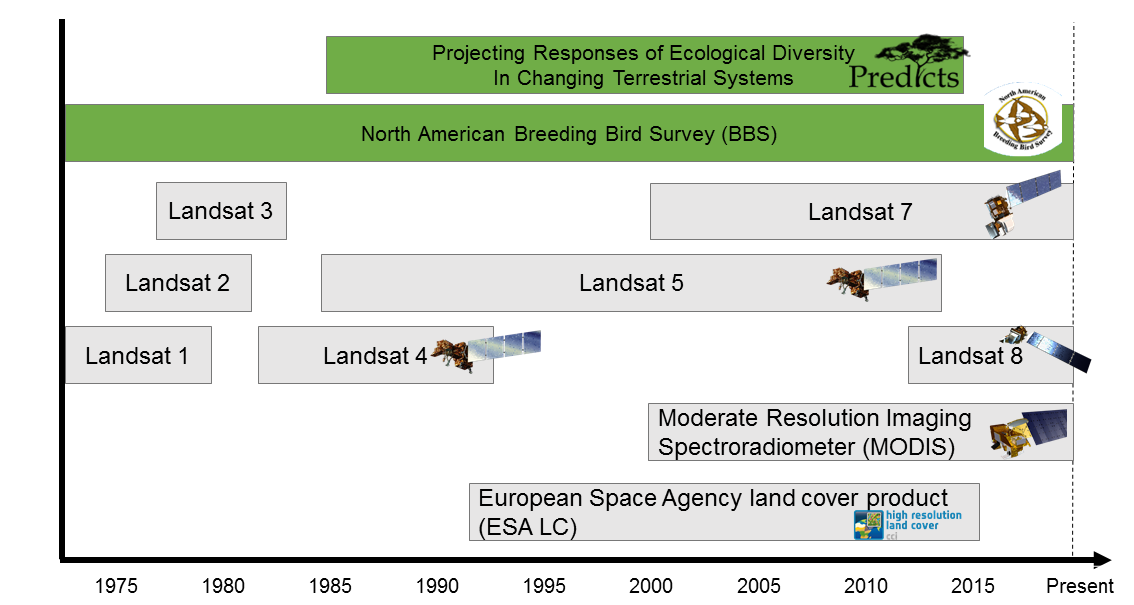
\includegraphics[width=1\textwidth]{chapter5/F01}
\caption{ (\textbf{a}) Schematic how landscape-wide land changes are quantified in a hypothetical BBS route. For each grid cell within the landscape (buffered circle around the BBS route) time series of annual March-June EVI were tested for a single or multiple land changes (see Methods \ref{C05_0203}). If a land change has been detected, we determined the position of all shifts in magnitude (abrupt loss in [“red”] or gain [“blue”]) or trends (greening [“dark green”] or browning [“brown”]) of photosynthetic activity (as measured by the EVI). (\textbf{b}) Changes in local bird diversity (as quantified by the GM and pBC) relative to a baseline year $y_0$ (highlighted in red) for an example BBS route. (\textbf{c}) Summarised proportion of all grid cells within the landscape with either a shift in magnitude or trend in EVI (colours as in \textbf{a}) per year. Map shown in the Albers equal area conic projection (NAD83).}
\label{F05_01}
\end{figure}
% -------------------------------------------- %

\subsection{Detection of landscape-wide land changes as changes in annual photosynthetic activity}
\label{C05_0203}

Landscape-wide land changes were quantified as the proportion of grid cells showing a shift in magnitude or trend of photosynthetic activity (Figure \ref{F05_01}\textbf{a}). Among all algorithms proposed to detect changes in remotely-sensed time series \citep{Zhu2017}, we relied on the generalized fluctuation framework originally developed for econometrics \citep{Bai2003,Zeileis2005}, later adapted for remote sensing as the Breaks for Additive Seasonal and Trend (BFAST) algorithm \citep{Verbesselt2010}. For each annual EVI time series, we tested for single or multiple structural breaks in linear trend using a recursive Moving Sum of Residuals (Rec-MOSUM) test over each four year window period \citep{Zeileis2005}. A statistically significant ($p < 0.05$) structural change test indicates whether at least a single structural break exists, in which case we iteratively fitted segmented linear regression models over the entire time series. The optimal number and position of all structural breaks were detected by minimizing both the Bayesian Information Criterion (BIC) and residual sum of squares (RSS) of the segmented regression models \citep{Zeileis2005,Verbesselt2010}. The framework requires a gap-free time series (“strucchange” package in R, ver. 1.5-1) and similar to previous studies we filled missing data using linear interpolation between adjacent years \citep{Verbesselt2010}.

Per grid cell and year, we differentiated all detected land change events as either abrupt shifts in magnitude or trend (Figure \ref{F05_01}). Shifts in magnitude were quantified using the predicted EVI data (from the segmented linear regression model) before and after the detected change date ($EVI_{After} - EVI_{Before}$) and categorized as either immediate loss or gain in photosynthetic activity in a given year if negative or positive, respectively. For shifts in trend, we assessed for each year whether the linear trend in annual EVI was significantly (p < 0.05) increasing (‘greening’), decreasing (‘browning’) or flat (‘stable’). Similarly, for time series with non-significant structural change tests, we fitted simple linear regression models to test whether the overall trend in EVI (across all 34 years) significantly increased or decreased.

For each BBS route and year (Figure \ref{F05_01}\textbf{c}), we summarized the amount of land that had either an abrupt shift in magnitude (loss or gain in EVI) or trend (greening or browning). Because the total land area differed among BBS routes, we calculated proportions relative to the total land area (see Methods \ref{C05_0202}). The change detection algorithm relies on a moving window (four years) and thus no land changes could be detected in the first (1984 - 1987) and last four (2014 - 2017) years of each EVI time series. In case a land change occurred within these years, the algorithm would set the date to the latest, respectively earliest, year possible (\eg 1987 and 2014) causing an inflated number of incorrectly dated land change events at the start and end of each time series. We therefore considered the first four years as ‘baseline’ (year\textunderscript{$0$}) and the last four as ‘overhang’ and removed them from further analyses. 

\subsection{Additional predictors and bird trait data}
\label{C05_0204}

At continental scales, bird diversity at BBS routes has been shown to be influenced by a number of environmental variables \citep{Rowhani2008,Goetz2014,Hobi2017,Barnagaud2017}. For a coarse measure of overall vegetation activity \citep{Rowhani2008,Hobi2017}, we calculated the mean EVI across all 34 years of annual Landsat composites per buffered BBS route (see Methods \ref{C05_0202}). Previous studies have shown that the number of bird species varies with elevation \citep{Jarzyna2017} and we extracted the mean     elevation of the buffered BBS route from the global GMTED (\textasciitilde $1$km resolution) product \citep{Danielson2011}. Precipitation-driven anomalies have been shown to affect the number and abundance of bird species \citep{Barnagaud2017}. We used the Standardized Precipitation-Evapotranspiration Index (SPEI), which quantifies anomalies relative to the conditions observed in a moving window before a given month \citep{Vicente-Serrano2010,Vicente-Serrano2012}. For each BBS route we extracted the monthly SPEI from SPEIbase \citep[ver. 2.5, \href{http://spei.csic.es}{http://spei.csic.es}, ][]{Vicente-Serrano2010} calculated on a climatology from 1901 to 2015 and over a moving window of three   months from January to March of each year \citep{Vicente-Serrano2010}, thus capturing precipitation anomalies in the winter months.

Similar to previous studies we used four functional trait groups \textendash\ nesting status, migratory behaviour, habitat guild and body mass \textendash\ to differentiate all bird species \citep{Schipper2016,Barnagaud2017}. Data on nesting (ground or canopy) and migratory behaviour (resident, short-distance and neotropical migrants) were obtained from \cite{Albright2011}, while data on bird species habitat guilds (\eg woodland, shrubland, grassland and urban birds) were extracted from the USGS website \href{https://www.mbr-pwrc.usgs.gov/bbs/guild/guildlst.html}{https://www.mbr-pwrc.usgs.gov/bbs/guild/guildlst.html}. The mean body mass (bm, measured in g) for all bird species was extracted from the Amniote database \citep{Myhrvold2015} and grouped into terciles of all estimates, \eg small, medium and large birds (bm < 33\%, bm $\geq$ 33\% \& bm < 66\%, bm $\geq$ 66\%). For species without trait estimates, we filled the missing data with the most common (mode) trait within the same bird genus, provided more than 50\% of all species within that genus had existing body mass estimates or identical categorical trait. For each BBS route and trait group we calculated separate GM estimates, but only for routes with at least 10 years of data and at least 3 different species within a trait group.

\subsection{Spatio-temporal models}
\label{C05_0205}

The aim of the statistical analyses was to investigate whether changes in local bird diversity (measured by GM and pBC) and landscape-wide land changes are correlated. To do so we relied on generalized additive regression models (GAMs), which are commonly used to model species population trends \citep{Fewster2000} and can handle complex non-linear, spatio-temporal and hierarchical datasets \citep{Kneib2009,Wood2011}. All considered variables were included as thin-plate smooth (fixed to 4 residual degrees of freedom to prevent overfitting) in the GAMs and we applied a smoothing penalization for variable selection \citep[mgcv parameter: select = TRUE]{Wood2008}. The approximate significance of non-linear model terms was assessed using an approach by \cite{Wood2013}. All GAMs were fitted using the ‘mgcv’ package \citep[ver. 1.8-24]{Wood2011} in R \citep[ver. 3.5.0]{RTeam2014}.

We distinguished between four groups of variables to be included as thin-plate smooths in the full GAM. (\textbf{1}) As “local” factors (f\textunderscript{local}) we considered the mean EVI, elevation and, for each year, the SPEI. (\textbf{2}) For landscape-wide land changes (f\textunderscript{landscape}), we included for each year the proportion (arcsine square root transformed) of abrupt shifts in magnitude (immediate loss and gain in EVI) and trend (browning or greening) in the landscape (Figure \ref{F05_01}\textbf{c}). (\textbf{3}) Incorporating spatial autocorrelation into regression models can improve predictive power \citep{Kneib2009,Dornelas2013}, especially when local biodiversity was surveyed over large scales such as the continental U.S. . We followed an approach by \citeauthor{Kneib2009} and included the spatial coordinates (f\textunderscript{spatial}) of each BBS route using a non-linear smooth surface function $g(x_{Northing},x_{Easting})$ with a tensor product P-spline \citep{Kneib2009}. Northing and easting coordinates were obtained by projecting the centroid of each buffered BBS route to an Albers equal area conic projection (NAD83). (\textbf{4}) For comparing biodiversity measures among BBS routes, species detectability or misidentification by different BBS observers has to be accounted for \citep{Sauer1994,Harris2018}. We included the BBS route ID (f\textunderscript{obs}) as random intercept in all models, therefore estimating the effect of f\textunderscript{local}, f\textunderscript{landscape} and f\textunderscript{spatial} on local biodiversity measures (GM and pBC) across all BBS routes. We acknowledge that using the route ID does not fully account for differences in observer abilities (there can be multiple observers for a single route), but previous studies found limited influence of varying observers over large scales \citep{Jarzyna2017,Barnagaud2017}. All biodiversity time series were detrended by including time (year) as linear predictor to avoid spurious correlations. To account for temporal autocorrelation, we included an autoregressive error structure (AR1), which we parametrized by visually assessing the autocorrelation function of the full model residuals at lag 1 ($\rho = 0.5$).

We tested if past (\eg the years before a BBS) landscape-wide land changes continued to influence bird diversity change in subsequent years. A ‘lagged’ correlation between two time series is commonly known as “Granger causality”, where one “time series $x_t$ contains information in past terms that helps the prediction of $y_t$“ \citep{Granger1969}. We followed an approach by \cite{Papagiannopoulou2017} and assessed the relative improvement in explanatory power of models including preceding instead of concurrent land changes. Preceding land changes with abrupt shifts in magnitude (loss or gain in EVI) of up to five years were included either individually, thus adding estimates for the preceding year $i = 1,...,5$ only; or cumulatively, where aggregated estimates for the preceding years $1:i$ were included in the model \citep{Jung2018}. The relative improvement in explanatory power was assessed using out-of-bag (OOB) coefficients of determination (R\textsuperscript{2}). To do so we split all time series into training and test datasets ($50/50$) 100 times at random. All models included the f\textunderscript{local} and f\textunderscript{spatial} variables to account for variation not directly attributable to landscape-wide land changes.

Lastly, we assessed the explanatory power of each group of variables (f\textunderscript{local}, f\textunderscript{spatial}, f\textunderscript{landscape}) spatio-temporally and for birds grouped by functional traits. To do so we fitted several GAMs using the GM (log-transformed) or pBC as response variable with a gaussian log-link distribution. We first fitted a “full” GAM including all variables, followed by separate GAMs where groups of variables (f\textunderscript{local}, f\textunderscript{spatial}, f\textunderscript{landscape}) were explicitly excluded from the model. Models for both GM and pBC converged well (Appendix Figure \ref{SI05_03}-\ref{SI05_04}), although the largest changes in pBC were generally poorly predicted by the models (Appendix Figure \ref{SI05_04}). The explanatory power of all models was assessed by calculating the R\textsuperscript{2} of each model. The group of variables (f\textunderscript{local}, f\textunderscript{spatial}, f\textunderscript{landscape}) explaining the most variation was then identified from the largest reduction (partial R\textsuperscript{2}, relative to the full model) in R\textsuperscript{2} \citep{Papagiannopoulou2017}. We assessed patterns of the most important group of variables spatially and in relation to robust linear trends in biodiversity measures \citep[fitted using the MASS package, ver. 7.3-49,][]{Venables2002}. Lastly, we investigated if the explanatory power of landscape-wide land changes (f\textunderscript{landscape}) varied with either bird species being differentiated by functional trait groups (see \ref{C05_0204}) or with BBS routes grouped by U.S. ecoregions \citep[Level 1,][]{Omernik1987}, which we derived by intersecting the centroid of each buffered BBS route with the U.S. ecoregions layer. For each functional trait group, we fitted two separate GAMs either including or excluding all f\textunderscript{landscape} variables before calculating the difference in R\textsuperscript{2} attributable to f\textunderscript{landscape} variables. For U.S. ecoregions we assessed the contribution of f\textunderscript{landscape} variables to the total R\textsuperscript{2} on overall GM change.

\section{Results}
\label{C05_03}

Both local bird diversity and landscapes have changed across the continental USA. Across all BBS routes the geometric mean of relative abundances (GM) increased by 0.01\% $\pm$ 0.002 standard error (SE) per year (mean first derivative) in the first two decades from 1984 to 2005, after which annual decreases of 0.01\% $\pm$ 0.003 SE were observed (Appendix Figure \ref{SI05_05}\textbf{a}). The compositional similarity of bird assemblages (pBC) decreased by 0.006\% $\pm$ 0.001 SE per year (Appendix Figure \ref{SI05_05}\textbf{b}). Landscapes surrounding each BBS route had on average 6\% $\pm$ 6.42 SD (range 0.02\% – 78.96\%) of land experiencing at least one land change in the period 1984 to 2017 (Appendix Figure \ref{SI05_06}). Over the same period a decrease in landscape-wide land changes were observed (mean robust linear trend = -0.00015 $\pm$ 0.0198 SD, range -0.545 to 0.112) but with large spatial variability (Appendix Figure \ref{SI05_07}). Across all BBS routes the mean proportion of land experiencing a land change with an abrupt shift in magnitude (loss or gain in EVI) fluctuated strongly (Appendix Figure \ref{SI05_08}\textbf{a}), while shifts in trend showed an inverse hump-shaped pattern for greening and a continuous decrease for browning (Appendix Figure \ref{SI05_08}\textbf{b}). Shifts in magnitude or trend were little correlated among each other (Appendix Figure \ref{SI05_09}) and across ecoregions (Appendix Figure \ref{SI05_10}).

% ---------------- Figure 2 --------------------- %
\begin{figure}[htb]
\centering
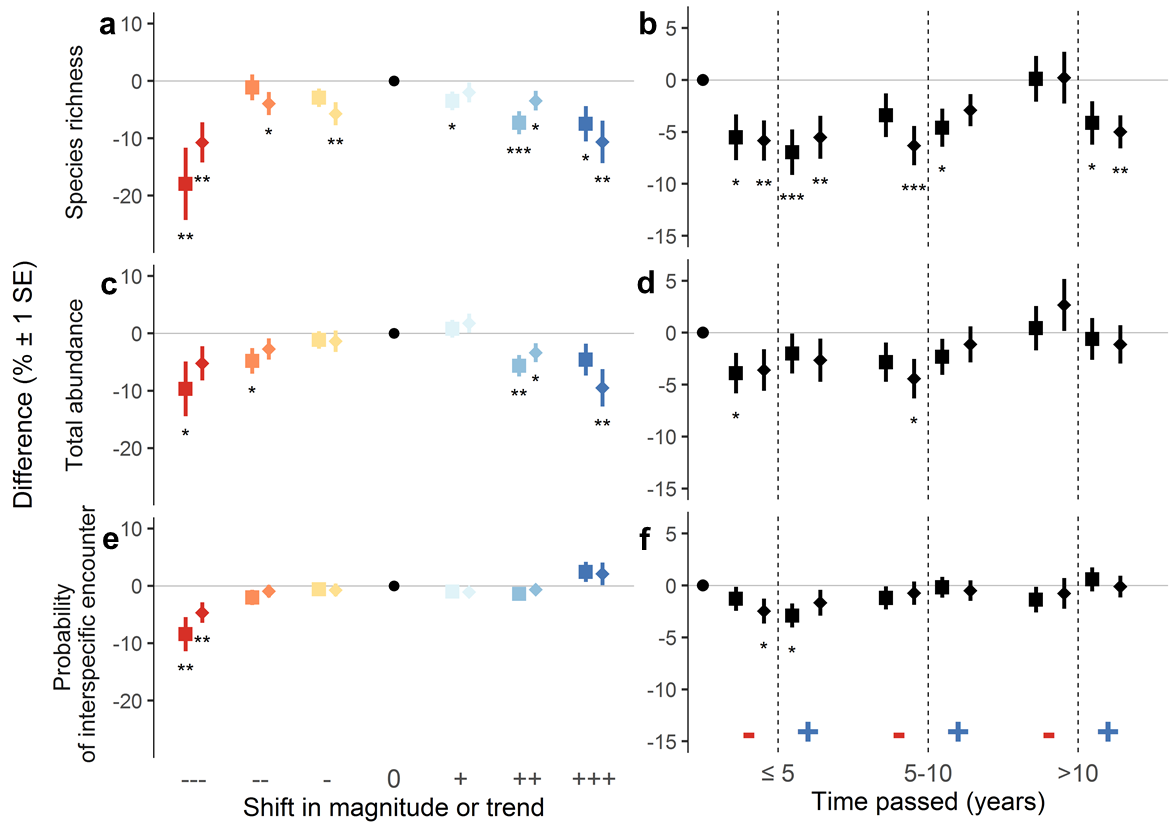
\includegraphics[width=1\textwidth]{chapter5/F02}
\caption{ Partial effects of landscape-wide land changes (proportion of landscape) per unit of change in (\textbf{a}) the geometric mean of relative abundance (GM) and (\textbf{b}) the progressive Bray-Curtis index (pBC). Colours indicate either abrupt shifts in magnitude with losses (red lines) or gains (blue) in EVI or trend with greening (green) or browning (brown) land. Error margins show the estimated standard error of the partial effect (grey shading) and rugs the observed proportion of landscape-wide land changes across all BBS routes. Flat lines without error margins indicate that the term was penalized out during model fitting and thus had no effect on the biodiversity measure. }
\label{F05_02}
\end{figure}
% -------------------------------------------- %

Bird diversity change is correlated with landscape-wide land changes. The GM significantly decreased ($F_{4} = 10.8, p < 0.001$) in years with a large proportion of landscape-wide abrupt gains of EVI (Figure \ref{F05_02}\textbf{a}, blue line). More landscape-wide abrupt losses of EVI led to a significant decrease in GM ($F_{4} = 6.44, p = 0.001$), but only after \textasciitilde 10\% of the landscape had abrupt losses in a given year (Figure \ref{F05_02}\textbf{a}, red line). The GM also decreased with more land in the landscape browning ($F_{4} = 37.89, p = 0.057$), while a high proportion of greening land in the landscape had no effect ($F_{4} = 0, p = 0.529$) on changes in GM (Figure \ref{F05_02}\textbf{a}). The pBC significantly increased with a large proportion of landscape-wide abrupt losses ($F_{4} = 8.25, p < 0.001$) or gains ($F_{4} = 0.614, p = 0.1$) in EVI (Figure \ref{F05_02}\textbf{b}). The pBC also increased with a large proportion of browning ($F_{4} = 13.81, p = 0.038$) or greening land ($F_{4} = 74.25, p = 0.005$) in the wider landscape (Figure \ref{F05_02}\textbf{b}).

Local factors strongly influence local bird biodiversity change. The GM significantly increased ($F_{4} = 1789.06, p < 0.001$, Appendix Figure \ref{SI05_11}\textbf{a}) and the pBC significantly decreased ($F_{4} = 1923.71, p < 0.001$, Appendix Figure \ref{SI05_11}\textbf{b}) at BBS routes of high mean elevation. GM significantly increased ($F_{4} = 291.05, p < 0.001$) in landscapes with overall low photosynthetic activity (EVI < 0.4) but decreased in landscapes with high photosynthetic activity; a pattern that was reversed for pBC (Appendix Figure \ref{SI05_11}). Years of abnormal precipitation between January and March had no effect on GM or pBC change (Appendix Figure \ref{SI05_11}).

Land changes in one year continued to influence local bird diversity in subsequent years. The mean explanatory power (out-of-bag [OOB] R\textsuperscript{2}) of abrupt shifts in magnitude in concurrent years (Lag 0, Figure \ref{F05_03}) was 0.03 (0.047 cumulatively) for GM and 0.126 (0.122) for pBC. A consideration of abrupt shifts in magnitude in preceding years explained modestly more variation than those in concurrent years (Figure \ref{F05_03}). The individual inclusion of one to five preceding years of abrupt shifts in magnitude explained similar amounts of variation (mean OOB R\textsuperscript{2} = 0.031) in GM, whereas for pBC only preceding abrupt shifts in magnitude more than three years ago increased explanatory power (mean OOB R\textsuperscript{2} = 0.129, Figure \ref{F05_03}). Considering cumulatively preceding abrupt shifts in magnitude increased the mean explanatory power for both GM and pBC (Figure \ref{F05_03}), although for pBC the relative improvement in explanatory power was highest at three cumulatively included preceding years (mean OOB R\textsuperscript{2} of year three = 0.128).

% ---------------- Figure 3 --------------------- %
\begin{figure}[htb]
\centering
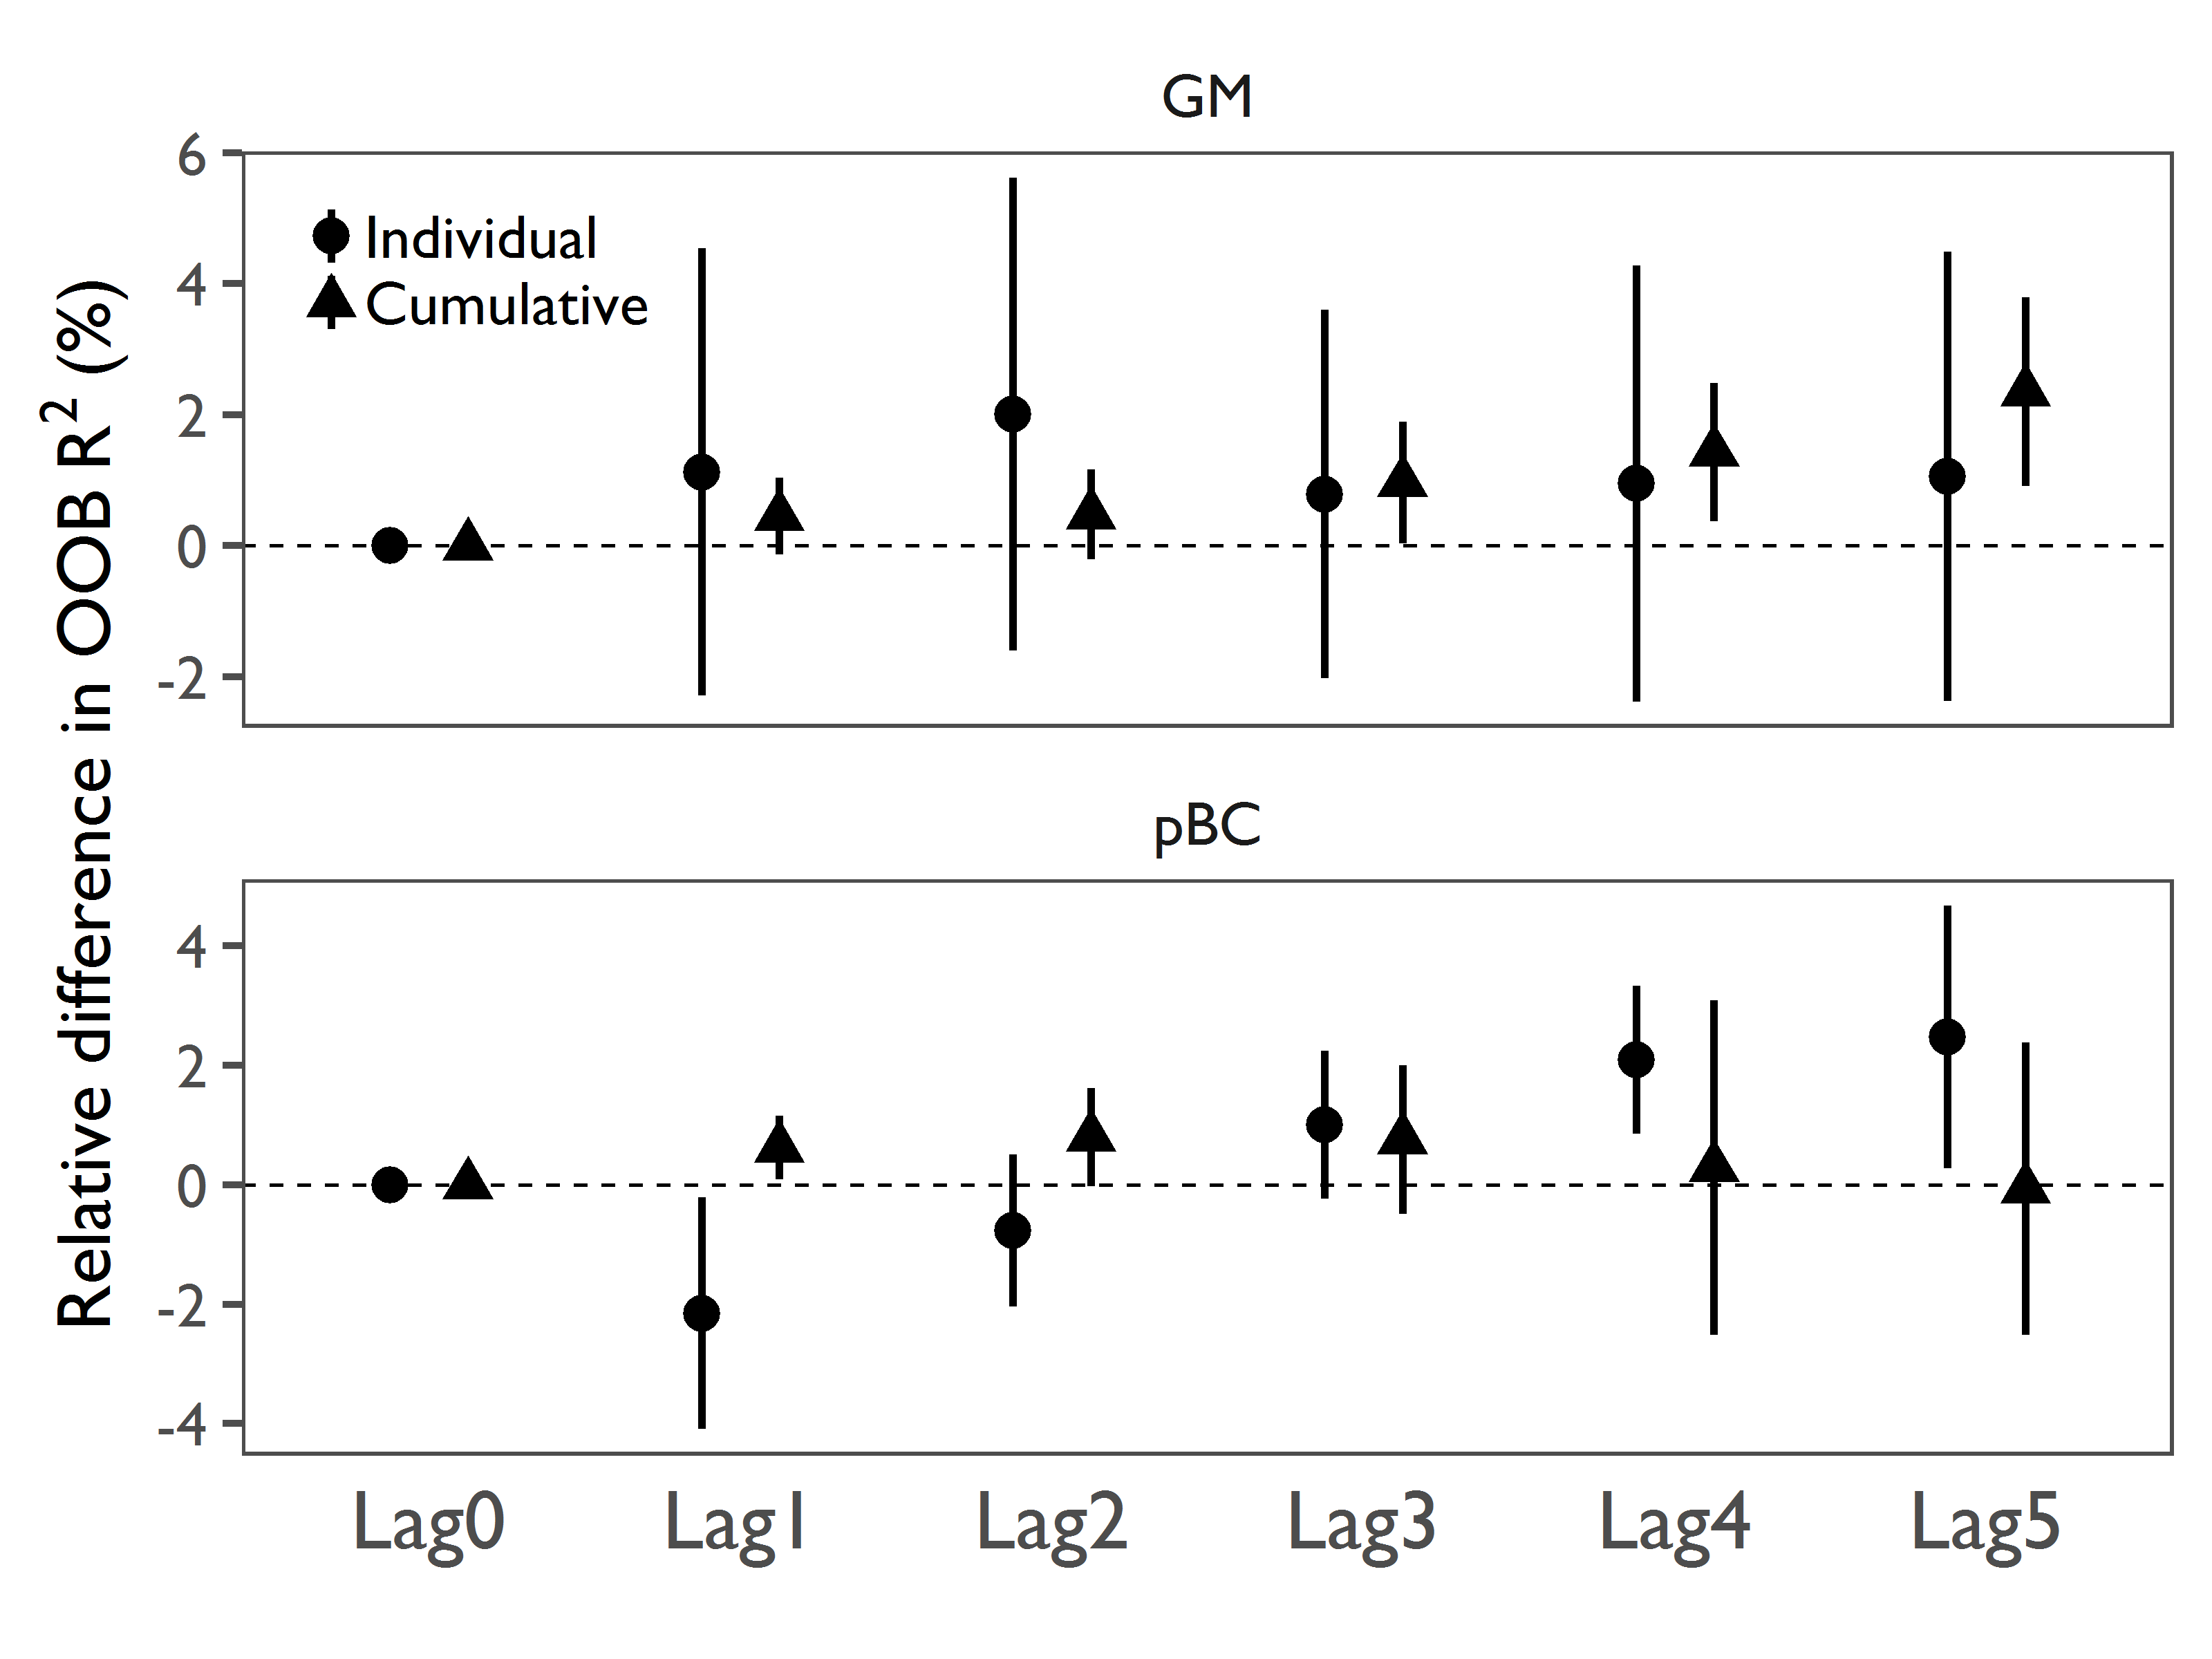
\includegraphics[width=1\textwidth]{chapter5/F03}
\caption{Preceding landscape-wide land changes of one to five years improve predictions of GM and pBC. Bird diversity time series for all BBS routes were randomly split (100 times) into training and test datasets and the explanatory power (R\textsuperscript{2}) was assessed relative to a model that only included concurrent abrupt shifts in magnitude (gain or loss of EVI) averaged across all random subsets. Symbols differentiate between two types of model structures, where past land changes were either added individually (circles) or aggregated cumulatively (triangles). Error bars show the standard deviation of the out-of-bag (OOB) R\textsuperscript{2} values. }
\label{F05_03}
\end{figure}
% -------------------------------------------- %

We assessed whether the explanatory power of all variables varied spatially (Figure \ref{F05_04}\textbf{a},\textbf{c}) and for linear trends of bird diversity change (Figure \ref{F05_04}\textbf{b},\textbf{d}). The full model including all variables explained 64.7\% of the total variation of changes in GM (69.3\% for pBC), with most of the variation explained by unknown differences among BBS routes (partial R\textsuperscript{2} of f\textunderscript{obs} = 58.5\%. for GM and 39.8\% for pBC). Of all variables considered, landscape-wide land changes were the most important predictor of GM change for 34.83\% of BBS routes (partial R\textsuperscript{2} range 0 – 54\%, Figure \ref{F05_04}\textbf{a}) and for pBC in 46.6\% of BBS routes (partial R\textsuperscript{2} range 0 – 7\%, Figure \ref{F05_04}\textbf{c}). Incidentally, landscape-wide land changes were the best predictor for some of the greatest changes (increase/decrease per year) in local bird diversity measures (Figure \ref{F05_04}\textbf{b},\textbf{d}).

% ---------------- Figure 4 --------------------- %
\begin{figure}[htb]
\centering
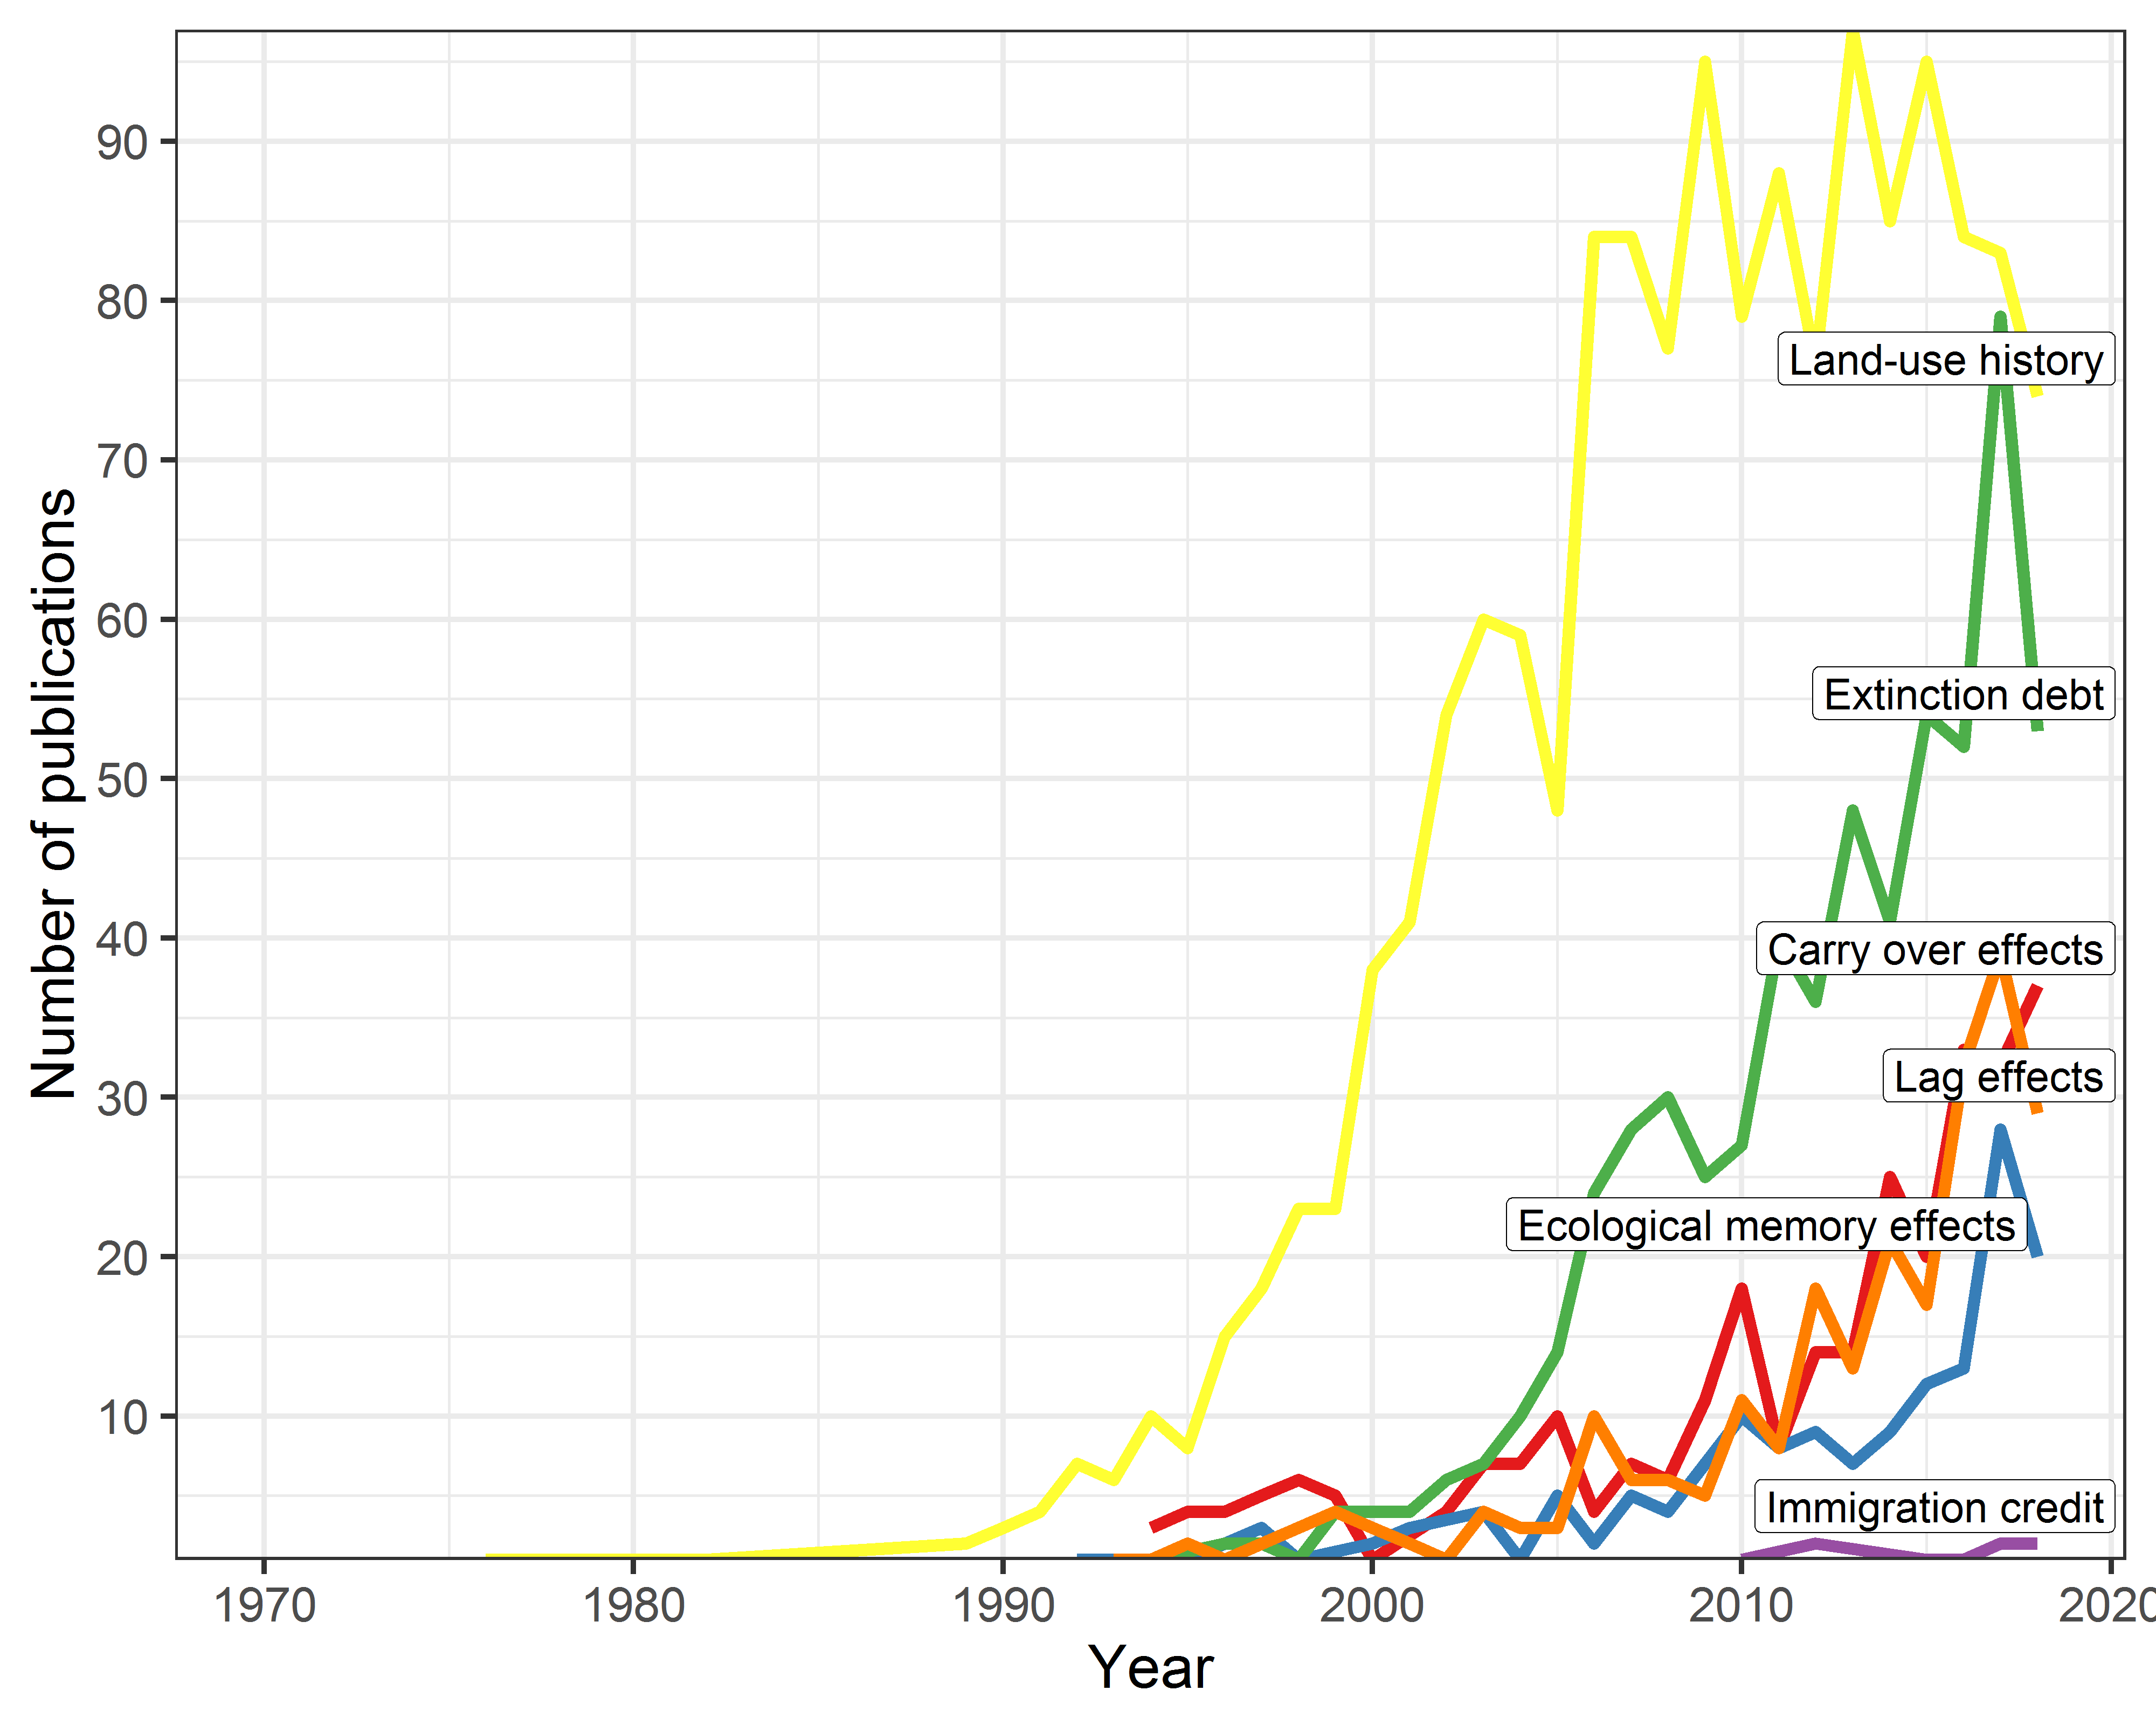
\includegraphics[width=1\textwidth]{chapter5/F04}
\caption{Most important group of variables explaining changes in the (\textbf{a}) GM and (\textbf{c}) pBC at 2745 BBS routes across the United States of America. Point sizes in (\textbf{a},\textbf{c}) indicate larger partial R\textsuperscript{2} of the most important variable group. Colours indicate which of the considered variable groups, f\textunderscript{local} (red), f\textunderscript{landscape} (blue) or f\textunderscript{spatial} (green), explained most of the variation (greatest partial R\textsuperscript{2}) in the full model. (\textbf{b},\textbf{d}) Partial R\textsuperscript{2} of the most important variable group averaged per increase or decrease (robust linear trend per year) in GM or pBC.  }
\label{F05_04}
\end{figure}
% -------------------------------------------- %

The explanatory power of landscape-wide land changes on changes in GM differed among bird species of varying functional traits and across ecoregions (Figure \ref{F05_04}, Appendix Figure \ref{SI05_12}). On average landscape-wide land changes did not explain (mean partial R\textsuperscript{2} = -.02 $\pm$ 0.09 SD) changes in GM for birds of varying trait groups (Figure \ref{F05_05}\textbf{a}). Similar to spatial patterns of the most important group of variables (Figure \ref{F05_04}), landscape-wide land changes were only important for a subset of BBS routes (Figure \ref{F05_05}\textbf{a}, blue outliers) in which they explained up to 71.9\% of the total R\textsuperscript{2}. For many BBS routes however the inclusion of landscape-wide land changes did not increase but decreased the R\textsuperscript{2} for explaining changes in GM (Figure \ref{F05_05}\textbf{a}, red outliers). A visual exploration could not identify any spatial patterns in these outlier BBS routes and there were also no distinguishable differences between ecoregions (Figure \ref{F05_05}\textbf{b}) and especially in Southern Semi-Arid Highlands landscape-wide land changes did not increase the explained variation in GM change, despite the on average large proportion of browning land (Appendix Figure \ref{SI05_10}).

% ---------------- Figure 5 --------------------- %
\begin{figure}[htb]
\centering
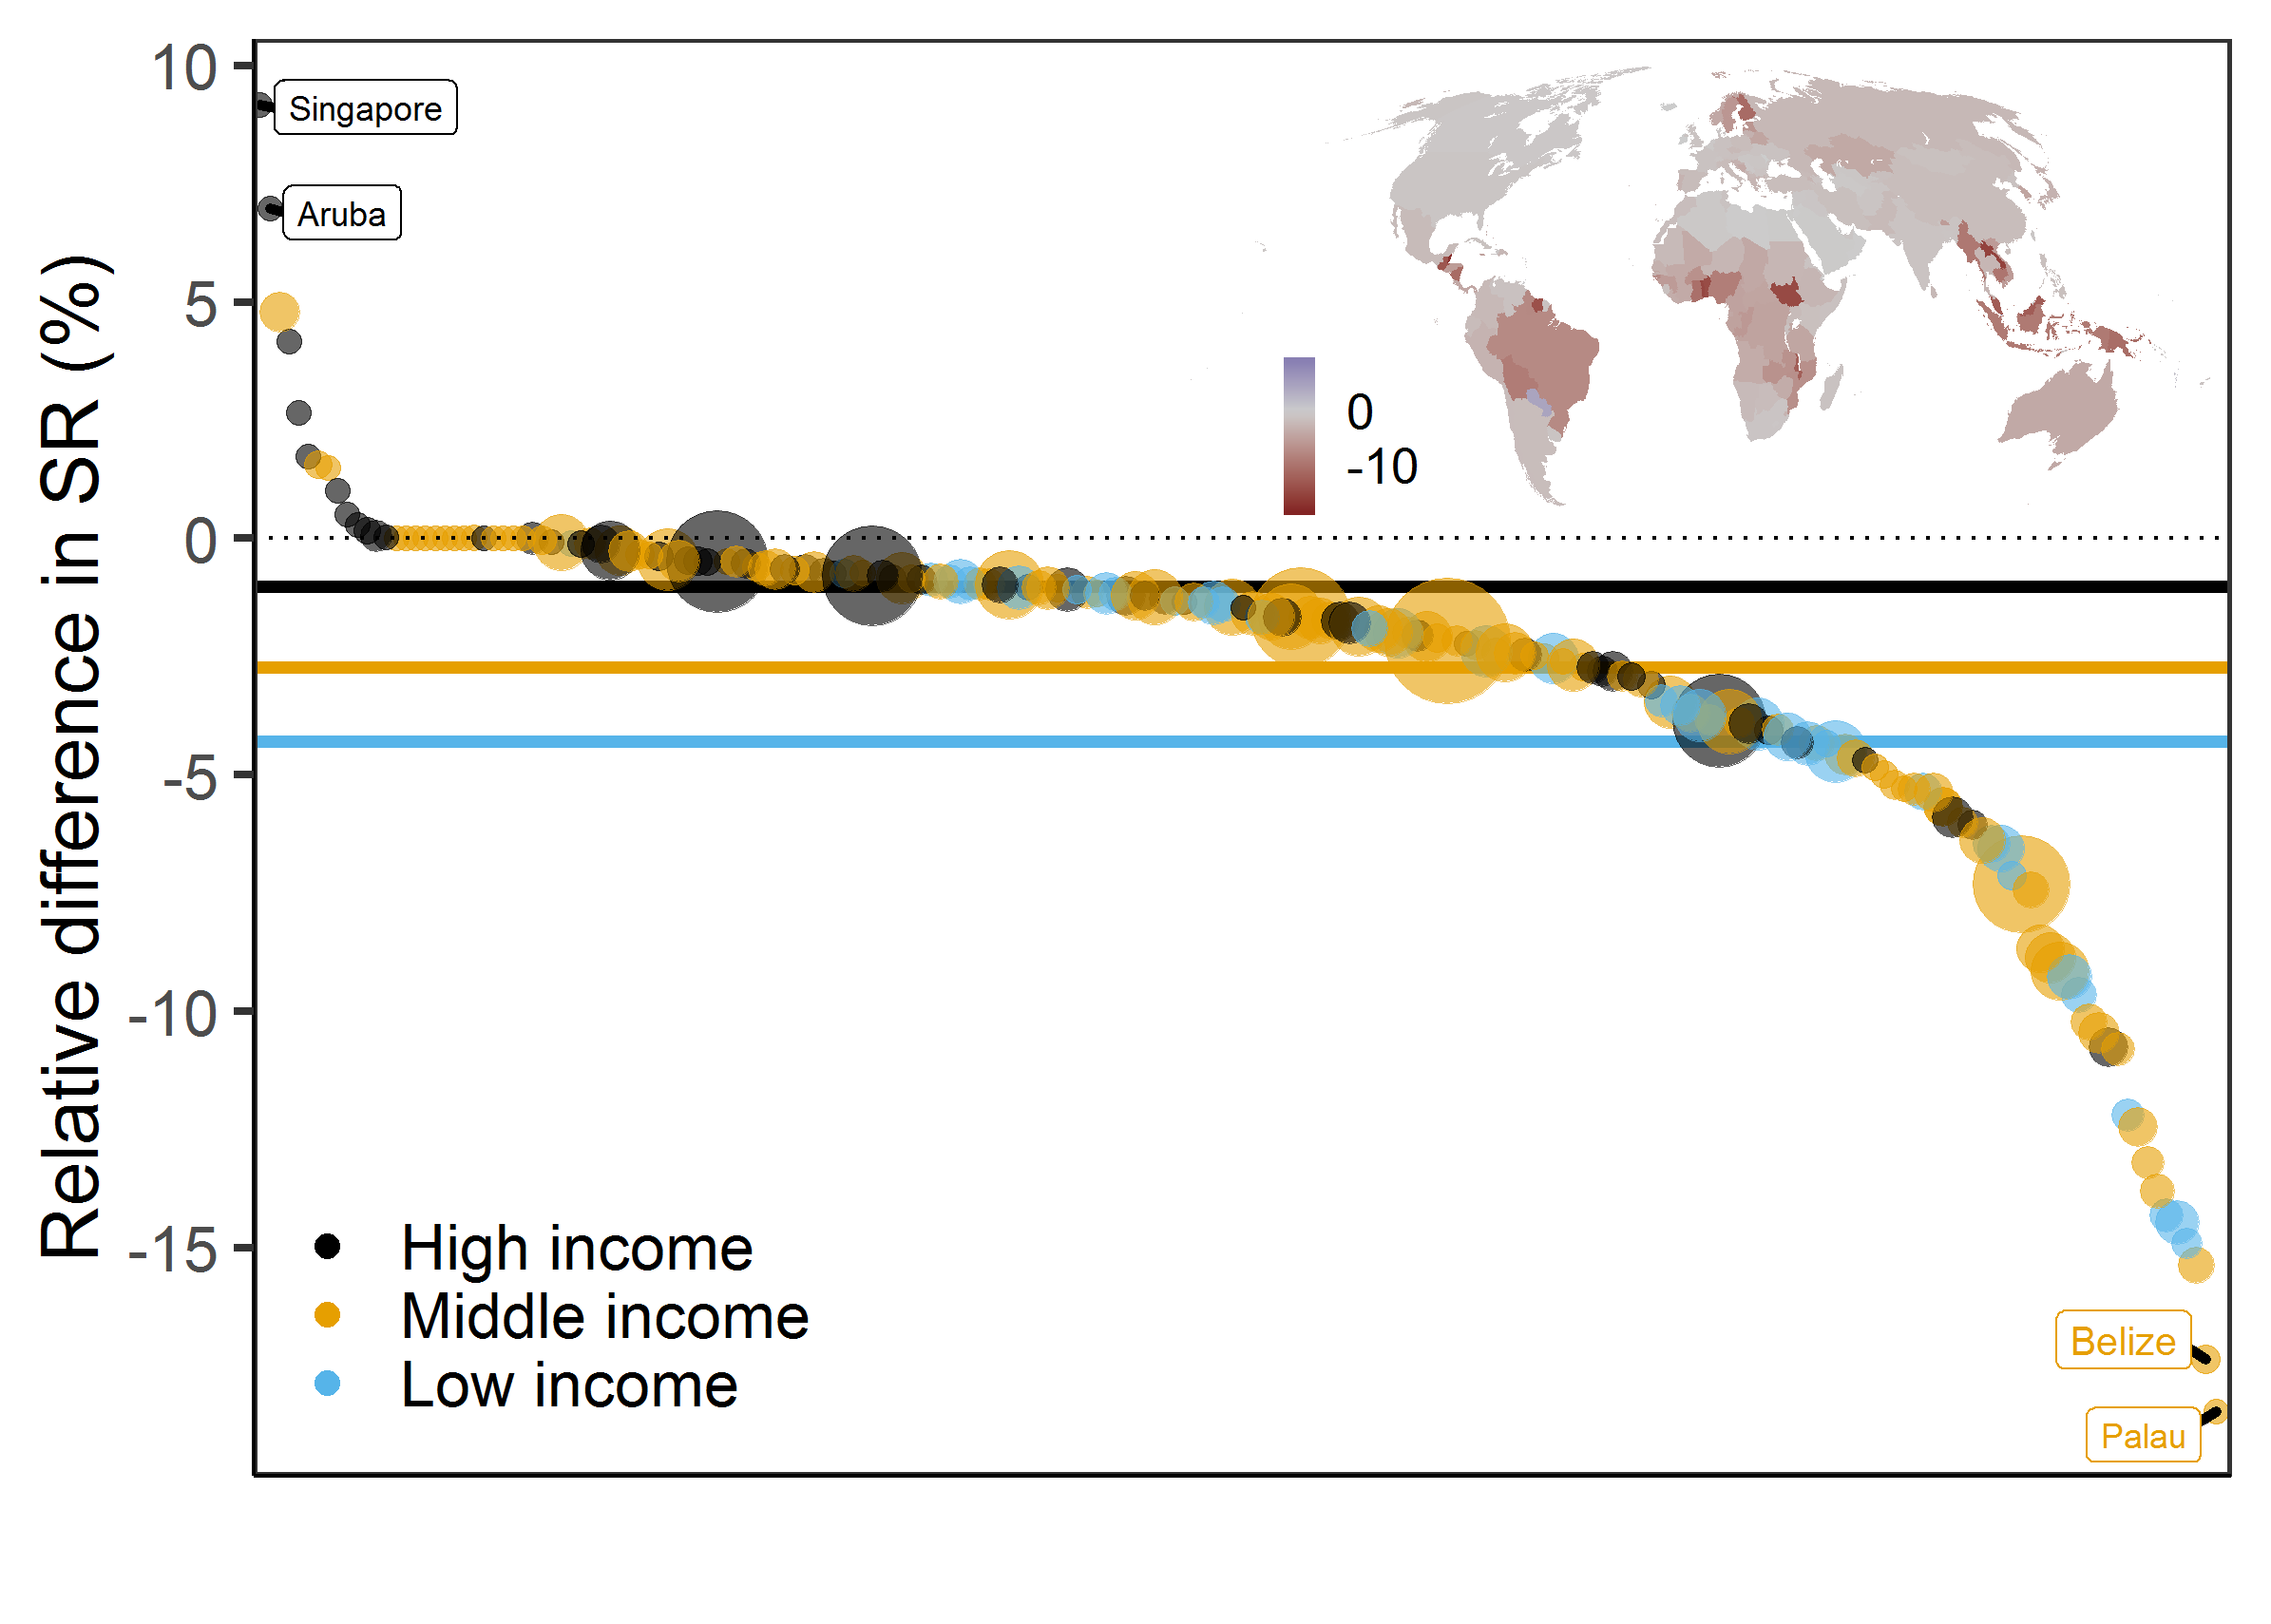
\includegraphics[width=1\textwidth]{chapter5/F05}
\caption{(\textbf{a}) Partial R\textsuperscript{2} of landscape-wide land changes (difference in explanatory power after excluding f\textunderscript{landscape} variables) for explaining changes in GM grouped by functional trait group. Shown is the distribution (grey), median and 50\% quantile (black) for each response variable. Red and blue points indicate outliers (1\% smallest / biggest partial R\textsuperscript{2} values). (\textbf{b}) Shows the absolute partial R\textsuperscript{2} of landscape-wide land changes in explaining trends in GM grouped by U.S. ecoregions. Coloured depending on whether landscape-wide land changes increased (blue) or decreased (red) overall R\textsuperscript{2}. Black points and error bars show the mean and standard error of the mean.}
\label{F05_05}
\end{figure}
% -------------------------------------------- %

\section{Discussion}
\label{C05_04}

The aim of this study was to investigate whether land changes (as measured by abrupt shifts in magnitude or trend of photosynthetic activity) in the landscapes surrounding the U.S. breeding bird survey (BBS) routes are correlated with changes in local bird diversity. We found that a greater proportion of landscape-wide abrupt shifts in magnitude was correlated with a decrease of the geometric mean of relative abundances \citep[GM, ][]{Buckland2011} and an increase in the progressive Bray-Curtis index \citep[pBC, ][]{Rittenhouse2010}. A greater proportion of browning land was correlated with a decrease in GM and an increase in pBC, while more greening land increased pBC only (Figure \ref{F05_02}). Confirming previous studies, some local factors (\eg mean elevation and photosynthetic activity) influenced local bird diversity change. Changes in GM and pBC were not only influenced by concurrent abrupt shifts in magnitude, but also by individual and cumulative effects of preceding land changes (Figure \ref{F05_03}). On average, landscape-wide land changes had high explanatory power (R\textsuperscript{2} > 0.1) only for a few selected routes without any clear pattern in space (Figure \ref{F05_04}), across trait groups (Figure \ref{F05_05}\textbf{a}) or ecoregions (Figure \ref{F05_05}\textbf{b}).  We discuss how these results link to previous studies of local biodiversity change and landscape ecology. 

\subsection{Landscape-wide land changes as drivers of biodiversity change}
\label{C05_0401}

Land changes have previously been linked to local biodiversity change \citep{Brooks2002,Ewers2013,Cousins2015}. Like previous studies at the local scale (Chapter \ref{C03} in this thesis), we found local biodiversity measures to be more affected by larger abrupt shifts in magnitude at the landscape scale (Figure \ref{F05_02}). A greater proportion of abrupt shifts in magnitude and trend (for ‘browning’) in the wider landscape were associated with a significant decline in the GM (Figure \ref{F05_02}\textbf{a}), potentially indicating local bird population collapse as fewer individuals across species are observed \citep{Loh2005,Buckland2011}. Meanwhile more abrupt shifts in magnitude and trend in the wider landscape increased the pBC (Figure \ref{F05_02}\textbf{b}). Because we found the GM to decline with a greater proportion of landscape-wide land changes, it is likely that the changes in pBC are caused by an increase in species richness, a pattern shown before for the BBS data \citep{Schipper2016}. Previous studies found compositional changes in bird assemblages to be particularly associated with changes in the occurrence of rare and specialist species, leading to a “homogenization” of assemblages \citep{McKinney1999,Olden2006a,Newbold2018}. It could be that landscape-wide land changes increase the heterogeneity of resources and bird habitats available, thus allowing a greater number of bird species, but fewer individuals overall, to   thrive \citep{Holt2009,Stein2014}, for instance through increased competition \citep{RandallHughes2007}. 

Changes in GM and pBC differed with local environmental gradients (Appendix Figure \ref{SI05_11}). Consistent with previous studies \citep{Lomolino2008,Jarzyna2017}, the GM increased at BBS routes of high elevation (Appendix Figure \ref{SI05_11}\textbf{a}), indicating that bird species increasingly utilize high elevation regions, likely because of climate change. Those species appear to be different from the species previously inhabiting BBS routes at high elevations, given the strong negative effect of elevation on pBC (Appendix Figure \ref{SI05_11}\textbf{b}). Furthermore, we found changes in GM to decrease and “flatten” in BBS routes with high average photosynthetic activity (EVI > 0.4, Appendix Figure \ref{SI05_11}\textbf{a}), in contrast to the pBC, which increased in BBS routes of high photosynthetic activity (Appendix Figure Appendix Figure \ref{SI05_11}\textbf{b}). This is in line with previous studies that demonstrated that BBS routes with high average photosynthetic activity have fewer bird individuals \citep{Barnagaud2017} but higher number of bird species \citep{Rowhani2008,Goetz2014}, which could drive changes in pBC. Similar to previous studies \citep{Barnagaud2017}, we found no strong effect of precipitation anomalies prior to a BBS on GM or pBC (Appendix Figure \ref{SI05_11}). 

\subsection{Lag effects of preceding land changes}
\label{C05_0402}

Land changes can have immediate and delayed impacts on local biodiversity \citep{Kuussaari2009,Hylander2013}. Theory suggests that \textendash\ single and cumulative \textendash\ preceding land changes are correlated with larger changes in local biodiversity \citep{Scheffer2001,Andersen2009,Watson2014,Ratajczak2018}. We demonstrated that considering preceding landscape-wide land changes helps explain local GM and pBC change (Figure \ref{F05_03}). Increasing explanatory power of individual preceding years could be linked to an average “ecological memory” effect for birds, particularly for the 4\textsuperscript{th} and 5\textsuperscript{th} year prior and changes in pBC (Figure \ref{F05_03}), and is similar to what has been shown for plant species \citep{Ogle2015}. The impacts of cumulative preceding land changes depended on their duration \citep{Essl2015} and frequency \citep{Watson2014,Ratajczak2018} and a recent study found that considering cumulative preceding \textendash\ relative to concurrent \textendash\ differences in land-surface conditions explained more variation in local species assemblage composition \citep{Jung2018}. Similarly, we find that a consideration of cumulative periods of preceding land changes assists in explaining differences in local biodiversity (Figure \ref{F05_03}). Preceding land changes may have affected the resources available to birds thus directly influencing their fitness and persistence in subsequent years \citep{Holt2009,Harrison2011,Ogle2015}.

Our understanding of “lagged” effects of land change on biodiversity change are still in their infancy. The majority of previous studies investigated climatic influences on richness and abundance change \citep{Albright2011,Lindstrom2013,Valtonen2013,Martay2017}, but little is known about the influence of past land change. \cite{Rittenhouse2012} investigated differences in the proportion of landscape-wide land cover on bird diversity, but only used bi-annual, thematically non-consistent estimates of land cover. Other studies investigated the link between preceding land change and local biodiversity \citep[Chapter \ref{C02}-\ref{C03} in this thesis, ][]{Jung2018}, but only for spatial differences in local biodiversity rather than biodiversity change \textit{per se}, which might mask lasting impacts \citep{Franca2016,DePalma2018}. We show that a consideration of preceding land change explains biodiversity change better than concurrent land change (Figure \ref{F05_03}), indicating a general biotic lag towards land change for bird diversity. Future studies could benefit from analysing impacts of preceding land change on both mean and variance of biodiversity change \citep{Leung2017,Christensen2018} as well as considering varying sequences of remotely-sensed land change \citep{Watson2014}.

\subsection{Variability in explanatory power in space and functional traits}
\label{C05_0403}

Quantifying local biodiversity change and identifying drivers of these changes is not trivial \citep{Dornelas2013,Cardinale2018}. Drivers of local biodiversity change are often unknown or cannot be reliably quantified \citep{Hallmann2017}. In an attempt to forecast local bird richness change, \cite{Harris2018} parametrized models with and without (‘na\"{i}ve’) including remotely-sensed photosynthetic activity and climatic data. Surprisingly, they found na\"{i}ve models to predict changes in bird richness better than those models including such variables, which they attributed to a lack of abrupt biodiversity changes. Opposed to bird richness, which has been found to be stable or increase in the BBS data \citep{Schipper2016}, we found GM and pBC to decline (Appendix Figure \ref{SI05_05}), but it is unclear what is driving those changes.

Bird biodiversity can be constrained by “thresholds” of land-surface conditions \textendash\ such as vegetation availability \textendash\ in the wider landscape \citep{Andersen2009,Gutzwiller2015}. A global review of threshold responses towards landscape-wide land changes suggests, that bird diversity is most affected if more than 27.9\% of the landscape is changing \citep{Melo2018}. With exception of a few BBS routes (Figure \ref{F05_04}, Appendix Figure \ref{SI05_06}), the average proportion of land changes within landscapes was only 6\% (Appendix Figure \ref{SI05_06}-\ref{SI05_07} \& \ref{SI05_10}), which could explain why f\textunderscript{landscape} variables in our models explained on average little variation in bird diversity change and were important in a few BBS routes only (Figure \ref{F05_04}). However, it could also be that impacts of landscape-wide land changes on bird diversity are poorly generalizable and depend on local context and functional traits of bird species. 

Changes in local bird diversity differ by functional trait groups \citep[Appendix Figure \ref{SI05_12},][]{Jarzyna2017,Barnagaud2017}. Yet, the explanatory power of landscape-wide land changes on bird diversity change did not vary by functional groups of traits (Figure \ref{F05_05}\textbf{a}). Many birds are migratory and as such are affected by human persecution and climatic anomalies on their migration paths \citep{Sanderson2006,Tottrup2012}. Although we did not find any difference in explanatory power between migratory and non-migratory birds (Figure \ref{F05_05}\textbf{a}), our analysis only considered land changes in bird breeding grounds with the location of wintering grounds being unknown. A distinction into habitat guilds also did not assist in identifying differences in explanatory power (Figure \ref{F05_05}\textbf{a}), which is surprising given the difference in trend between for instance woodland and grassland birds (Appendix Figure \ref{SI05_12}). It could be that land changes specific to certain bird habitats, \eg changes in vegetation height \citep{Goetz2014}, are a better predictor of bird diversity change. 

In this study we investigated the influence of landscape-wide, rather than local, land changes on biodiversity change. Landscapes surrounding the BBS routes are constantly changing (Appendix Figure \ref{SI05_06}-\ref{SI05_07}) and such changes are expected to influence local biodiversity \citep{Manning2009,Turner2015,Seppelt2016}. However, the processes influencing local biodiversity at the landscape scale are difficult to quantify \citep{Chase2003}, dependent on spatial scale \citep{Miguet2015} and local context (elevation, terrain, climatology). Regular natural disturbances \textendash\ such as wild fires \textendash\ can occur in many U.S. ecoregions \citep{Morgan2001}, but there were only marginal differences in the explanatory power of landscape-wide land changes among U.S. ecoregions (Figure \ref{F05_05}\textbf{b}). Possibly bird diversity change is primarily driven by land changes not detectable in annual remotely-sensed photosynthetic activity and requires different remotely-sensed information \citep{Zhu2014,Goetz2014}. Overall, for most BBS routes, the drivers explaining local bird diversity change remain unknown (Figure \ref{F05_04}-\ref{F05_05}) and we suggest future studies to consider alternative attributes of remotely-sensed land change at the landscape-scale \citep{Watson2014} or other spatio-temporal variables not quantifiable from optical remote sensing.

\subsection{Conclusion}
\label{C05_0404}

Overall our results indicate that landscape-wide land changes are correlated with (Figure \ref{F05_02}) but did on average not explain bird diversity change across spatial scales (Figure \ref{F05_04}), functional groups (Figure \ref{F05_05}\textbf{a}) and ecoregions (Figure \ref{F05_05}\textbf{b}). Preceding land changes assisted in explaining changes in bird diversity (Figure \ref{F05_03}), highlighting the importance of biotic lag effects. We demonstrate that measures of biodiversity change are correlated with remotely-sensed landscape-wide land changes and highlight the need to better understand drivers of biodiversity change. Future studies investigating biodiversity change should consider changes in other remotely-sensed variables or variables not quantifiable through remote sensing (\eg pesticide use, human persecution, etc.). We furthermore suggest that more research is needed on scale-dependent effects (local vs landscape changes) of biodiversity change. 

\clearpage
%\bibliography{content/04Chapter}

%\appendix
%\begingroup
%  % SI - Figure 1 Missing data
\begin{figure}[h]
\centering
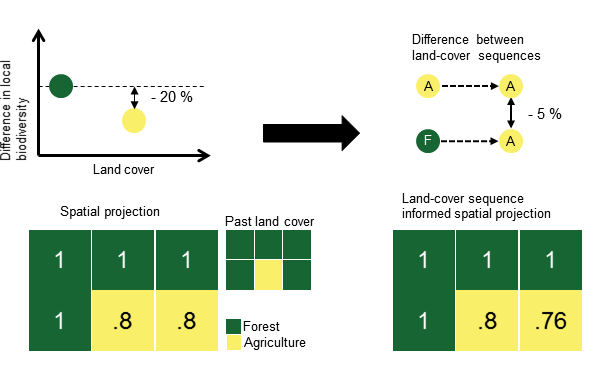
\includegraphics[width=1\textwidth]{chapter3/SI01}
\caption{ Average temporal distribution of Landsat data and an example times series of Landsat data. (\textbf{a}) Distribution of available Enhanced Vegetation Index (EVI) data in years covered by the Landsat missions. Points show the average monthly EVI data availability per year (0 to 12 months of data) across time series and PREDICTS sites grouped by 15\textdegree latitude bins. The size of points indicates the mean data availability (0 to 100\% with 100\% having 12 months of available data in a given year), while the colour shows the number of PREDICTS sites contributing to the mean (as PREDICTS sites were sampled in varying years). (\textbf{b}) Example time series for one PREDICTS site with a high proportion of missing data before 1999. In all analyses such time series were truncated to the period from 1999 onwards (indicated by the dashed line).}
\label{SI03_01}
\end{figure}

% SI - Figure 2 Binning
\begin{figure}[h]
\centering
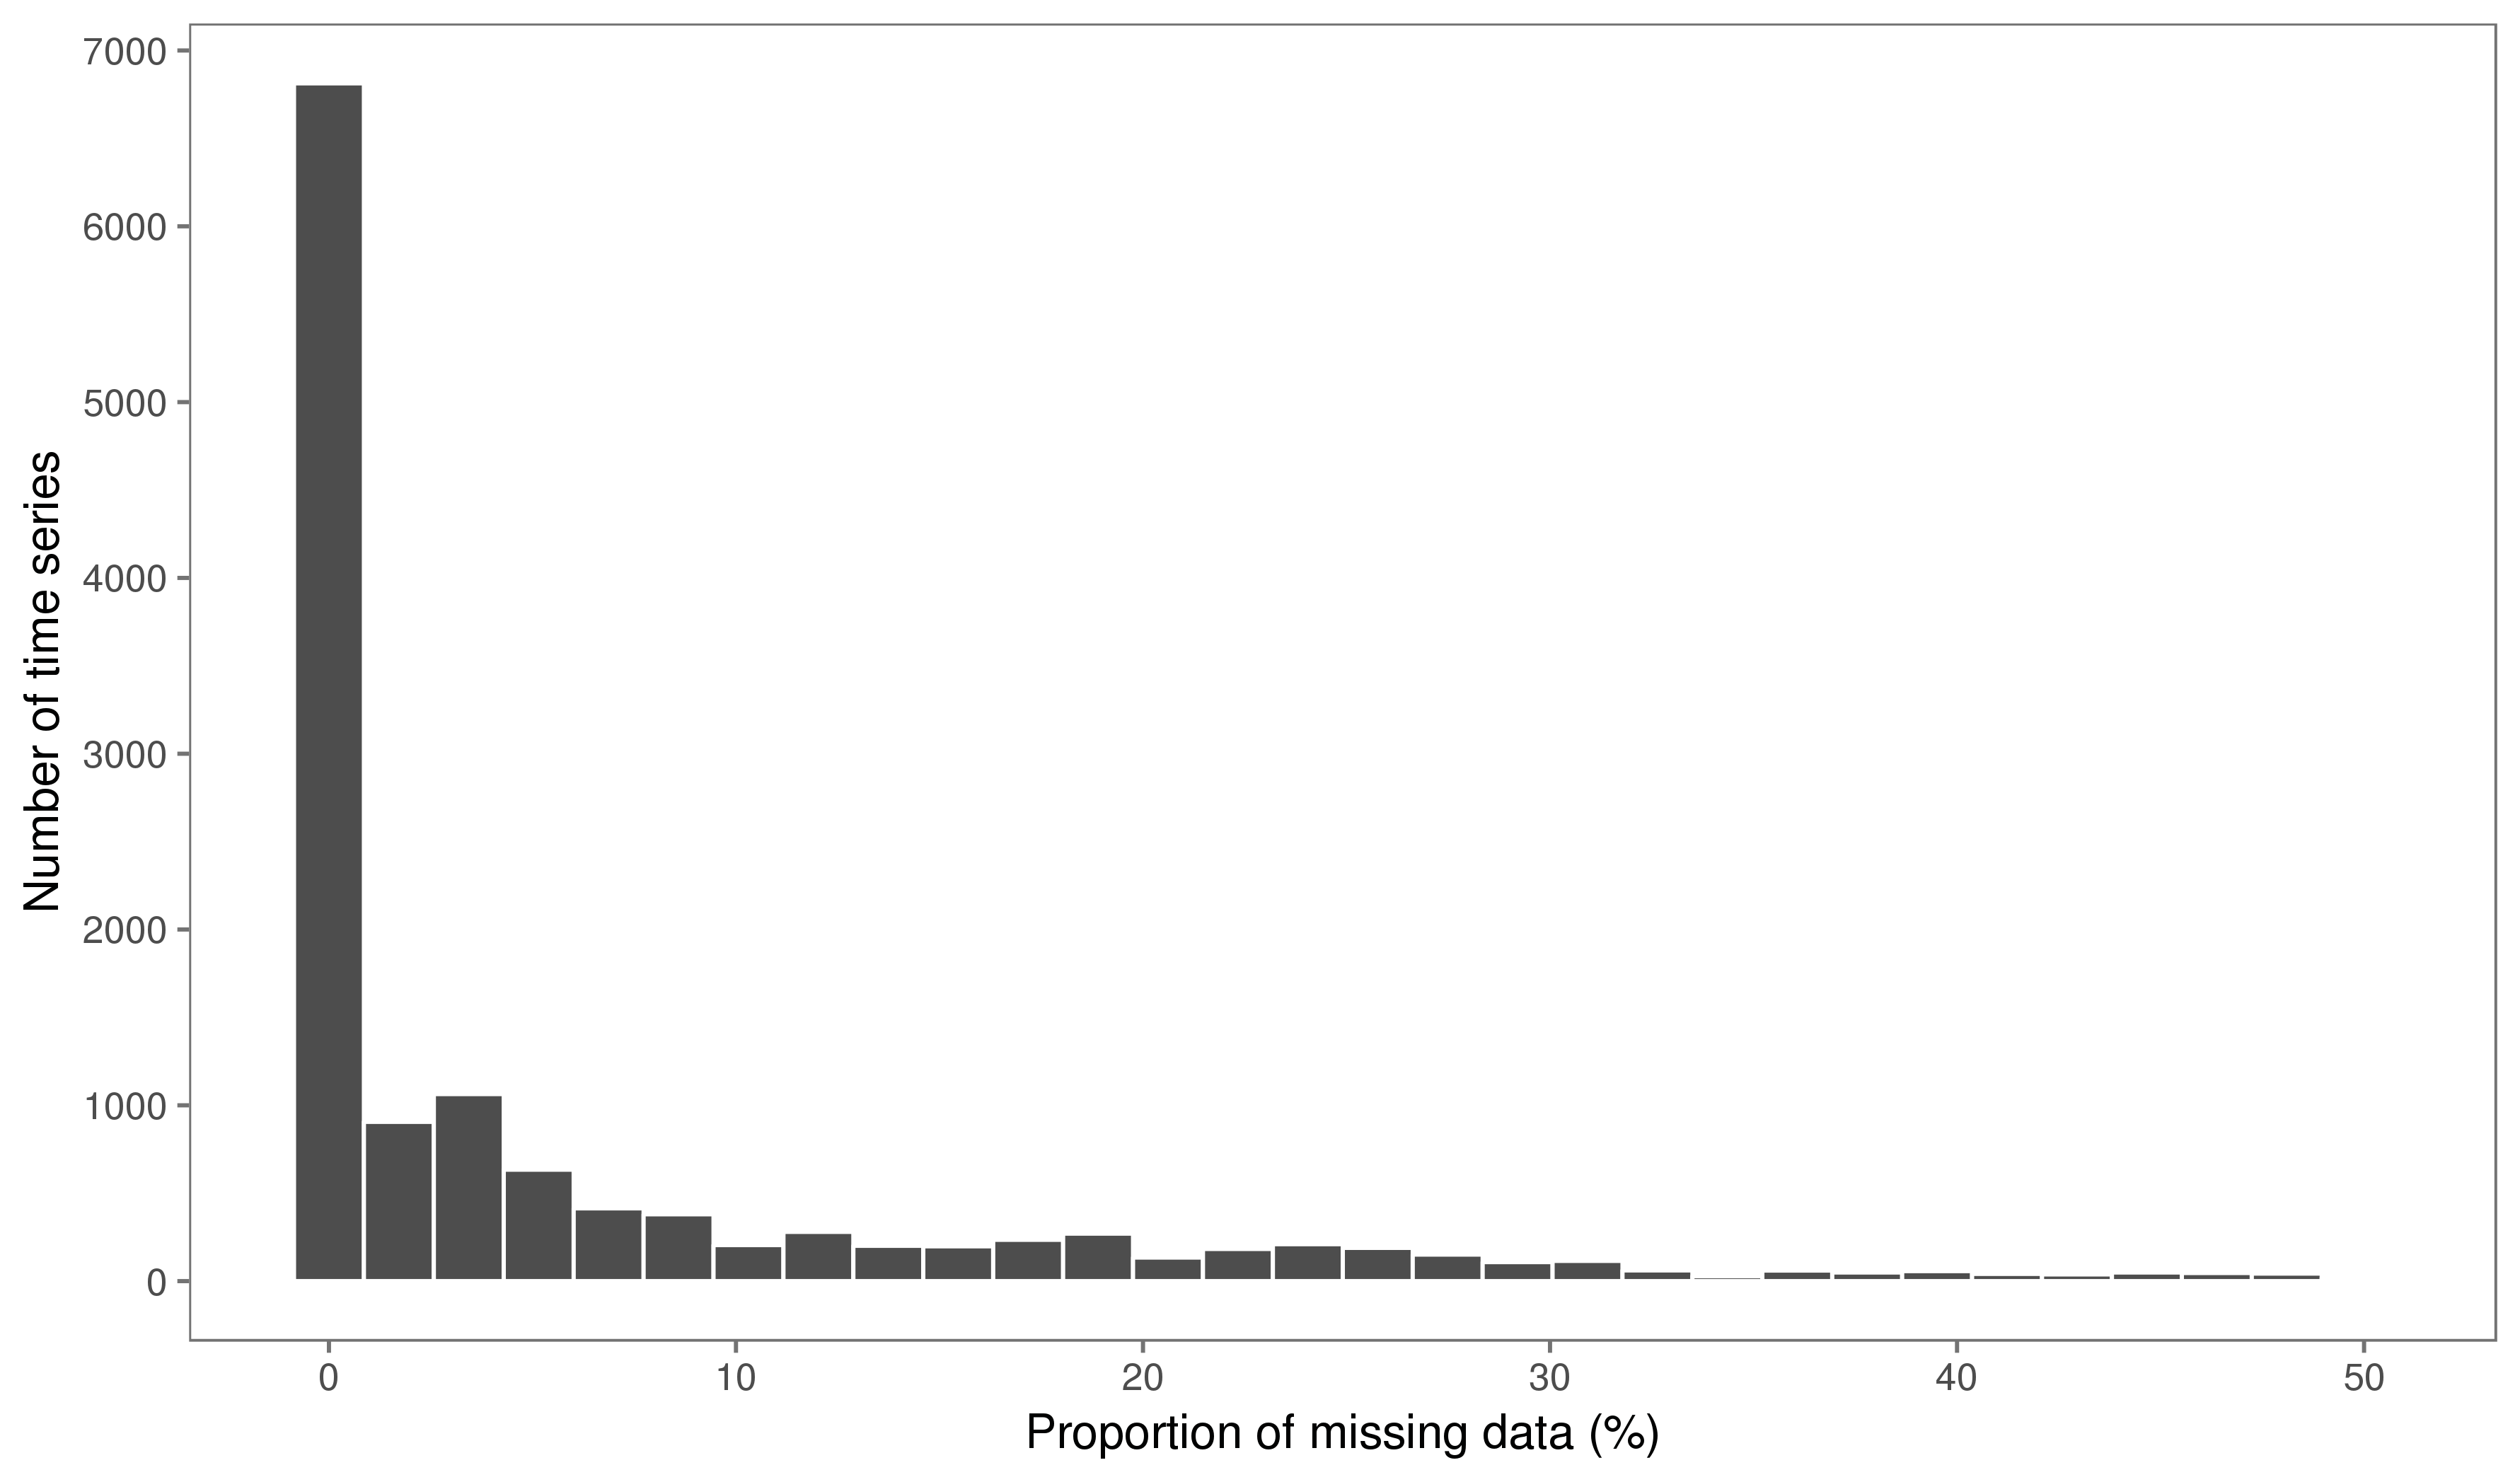
\includegraphics[width=1\textwidth]{chapter3/SI02}
\caption{ Number of sites with abrupt land change per attribute. Number of sites (black line) per attribute of abrupt land change with (\textbf{a}) the relative shift in magnitude, (\textbf{b}) the shift in trend as difference in annual EVI trend, and (\textbf{c}) the time passed between abrupt land change and biodiversity sampling. Background colours in (\textbf{a}) and (\textbf{b}) indicate the binning into six groups for shifts in magnitude (> 50\%, > 25\% to $\leq$ 50\%, and $\leq$ 25\% EVI loss [$---$ to $-$] or gain [$+++$ to $+$]), and in trend (0.01, 0.05, and > 0.05 annual negative [$---$ to $-$] to positive [$+++$ to $+$] EVI trend differences). Gray lines in (\textbf{c}) delineate bins of time passed ($\leq$ 5 years, > 5 and $\leq$ 10 years, and >10 years). Colours as in Figure \ref{F03_02}.}
\label{SI03_02}
\end{figure}

% SI Table 1------ %
% From here https://www.tablesgenerator.com/
\begin{table}[]
\centering
\caption{Number of PREDICTS sites and studies with an abrupt land change. Shown as either a change in magnitude (columns) and/or change in trend (trend). Symbols as in Figure \ref{F03_02}. }
\label{SIT03_01}
\begin{tabular}{@{}lllllllllll@{}}
                                          &                                           & \multicolumn{7}{c}{\textbf{Shift in magnitude}}                                                                                                                                                                    &                               &                             \\
                                          &                                           & \textbf{- - -}             & \textbf{- -}                & \textbf{-}                   & \textbf{0}                    & \textbf{+}                   & \textbf{+ +}                & \textbf{+ + +}              & \textbf{Total sites}          & \textbf{Studies}            \\ \cmidrule(l){3-11} 
                                          & \multicolumn{1}{l|}{- - -}                & 2                          & 8                           & 192                          & NA                            & 73                           & 26                          & 22                          & \cellcolor[HTML]{EFEFEF}323   & \cellcolor[HTML]{C0C0C0}57  \\
                                          & \multicolumn{1}{l|}{- -}                  & 7                          & 281                         & 642                          & NA                            & 497                          & 158                         & 53                          & \cellcolor[HTML]{EFEFEF}1638  & \cellcolor[HTML]{C0C0C0}175 \\
                                          & \multicolumn{1}{l|}{-}                    & 7                          & 88                          & 256                          & NA                            & 231                          & 154                         & 53                          & \cellcolor[HTML]{EFEFEF}789   & \cellcolor[HTML]{C0C0C0}184 \\
                                          & \multicolumn{1}{l|}{0}                    & NA                         & NA                          & NA                           & 10102                         & NA                           & NA                          & NA                          & \cellcolor[HTML]{EFEFEF}10102 & \cellcolor[HTML]{C0C0C0}358 \\
                                          & \multicolumn{1}{l|}{+}                    & 9                          & 102                         & 399                          & NA                            & 410                          & 205                         & 49                          & \cellcolor[HTML]{EFEFEF}1174  & \cellcolor[HTML]{C0C0C0}237 \\
                                          & \multicolumn{1}{l|}{\textbf{+ +}}         & 47                         & 172                         & 342                          & NA                            & 465                          & 254                         & 86                          & \cellcolor[HTML]{EFEFEF}1366  & \cellcolor[HTML]{C0C0C0}224 \\
\multirow{-7}{*}{\textbf{\rotatebox{90}{Shift in trend}}} & \multicolumn{1}{l|}{\textbf{+ + +}}       & 12                         & 137                         & 47                           & NA                            & 34                           & 12                          & 31                          & \cellcolor[HTML]{EFEFEF}273   & \cellcolor[HTML]{C0C0C0}56  \\
                                          & \multicolumn{1}{l|}{\textbf{Total sites}} & \cellcolor[HTML]{EFEFEF}84 & \cellcolor[HTML]{EFEFEF}788 & \cellcolor[HTML]{EFEFEF}1878 & \cellcolor[HTML]{EFEFEF}10102 & \cellcolor[HTML]{EFEFEF}1710 & \cellcolor[HTML]{EFEFEF}809 & \cellcolor[HTML]{EFEFEF}294 &                               &                             \\
                                          & \multicolumn{1}{c|}{\textbf{Studies}}     & \cellcolor[HTML]{C0C0C0}34 & \cellcolor[HTML]{C0C0C0}135 & \cellcolor[HTML]{C0C0C0}246  & \cellcolor[HTML]{C0C0C0}358   & \cellcolor[HTML]{C0C0C0}263  & \cellcolor[HTML]{C0C0C0}171 & \cellcolor[HTML]{C0C0C0}83  &                               &                            
\end{tabular}
\end{table}
% ------ %

% SI - Figure 3 Cross-correlations
\begin{figure}[h]
\centering
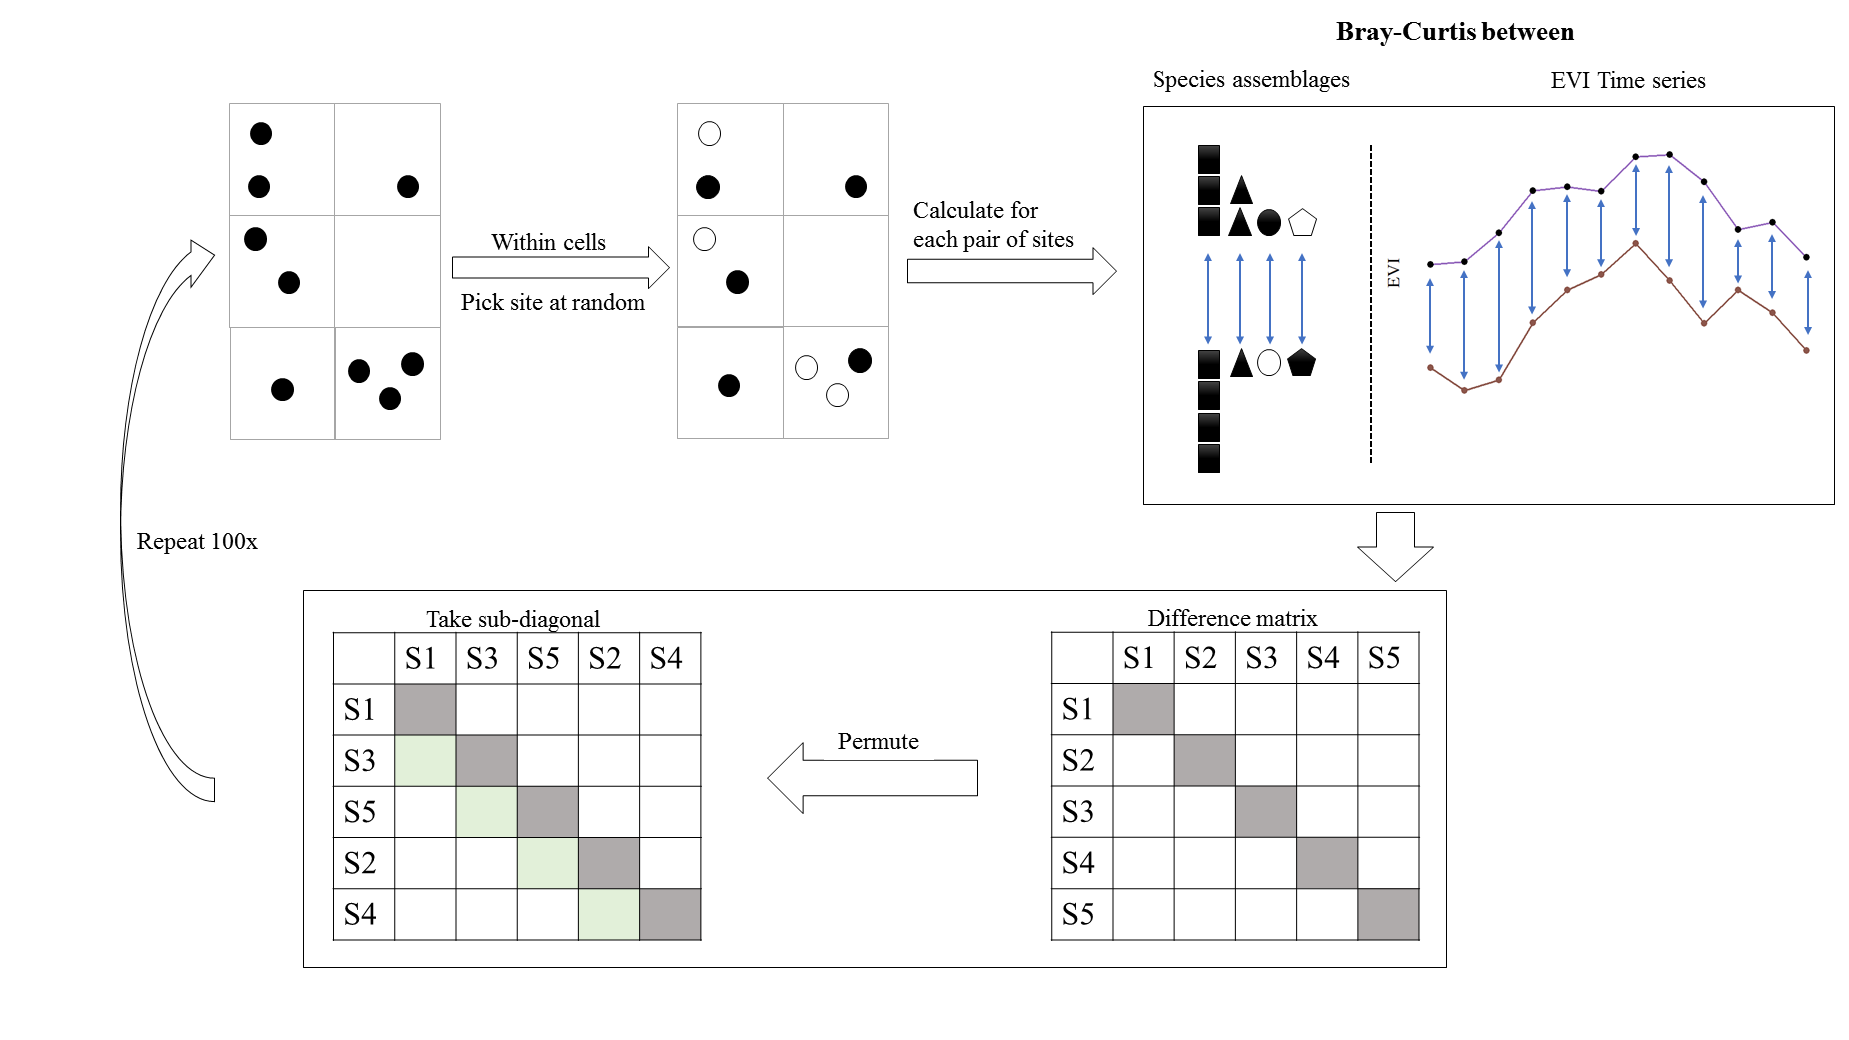
\includegraphics[width=1\textwidth]{chapter3/SI03}
\caption{ Correlations between attributes of abrupt land change. Showing shifts in magnitude, trend and time passed (see Methods). The lower facets show a point density plot, the upper facets the Pearson correlation coefficient between pairs of attributes and the diagonal a density plot.}
\label{SI03_03}
\end{figure}

%\endgroup
